\documentclass[11pt,a4paper]{article}

\usepackage{fullpage}
\usepackage{listings}
\usepackage{hyperref}
\usepackage{graphicx}
\usepackage{amsmath}
\usepackage{booktabs}
\usepackage{tabu}
\usepackage{titlesec}
\usepackage{fancyhdr}
\usepackage{color}
\usepackage{xcolor, colortbl}
\pagestyle{fancy}
\fancyhf{}
\usepackage{todonotes}                %% notes from the authors

\setcounter{secnumdepth}{4}
\renewcommand{\headrulewidth}{0pt}
\renewcommand{\footrulewidth}{0pt}
\newcommand{\num}[1]{\texttt{#1}}

\fancypagestyle{firstpagefooter} {
	\lfoot{\tiny{Version: 25.09.2018}}
	\cfoot{}
	\rfoot{\thepage}
	
}

\definecolor{mygreen}{rgb}{0,0.6,0}
\definecolor{mygray}{rgb}{0.82, 0.82, 0.82}

\lstset{
   basicstyle=\fontsize{9}{11}\selectfont\ttfamily,
   language=Python,
   commentstyle=\color{mygreen},    % comment style
}

\lfoot{Name: Stefano Peverelli Legi: 19-980-396}
\rfoot{\thepage}

\begin{document}

\title{Advanced Systems Lab Report\\ \normalsize{Autumn Semester 2018}}
\author{Name: Stefano Peverelli\\Legi: 19-980-396}
\date{
	\vspace{4cm}
	\textbf{Grading} \\
	\vspace{0.5cm}
	\begin{tabular}{|c|c|}
		\hline  \textbf{Section} & \textbf{Points} \\
		\hline  1                &                 \\ 
		\hline  2                &                 \\ 
		\hline  3                &                 \\ 
		\hline  4                &                 \\ 
		\hline  5                &                 \\ 
		\hline  6                &                 \\ 
		\hline  7                &                 \\ 
		\hline \hline Total      &                 \\
		\hline 
	\end{tabular} 
}
\maketitle
\thispagestyle{firstpagefooter}

\newpage

\section{System Overview (75 pts)}

Following is a description of the class structure of the Middleware:

\begin{itemize}
    \item \texttt{MW} - responsible for accepting incoming socket connections, instantiating the \texttt{Writer} threads, and for enqueuing each request.
    \item \texttt{Request} - this class represent a request object, it contains the request's type and measures (presented below).
    \item \texttt{Worker} - each \texttt{Worker} establishes a socket connection with the memchached servers, dequeues a request, performs load balancing, and process the request (sends to servers, handle responses and collects some statistics.
    \item \texttt{Statistic} - container for all measured statistics.
    \item \texttt{Writer} - when shutting down the Middleware, it collects all the statistics from each \texttt{Worker}, aggregates them and save them to disk.
\end{itemize}

\begin{figure}[h]
    \centering
    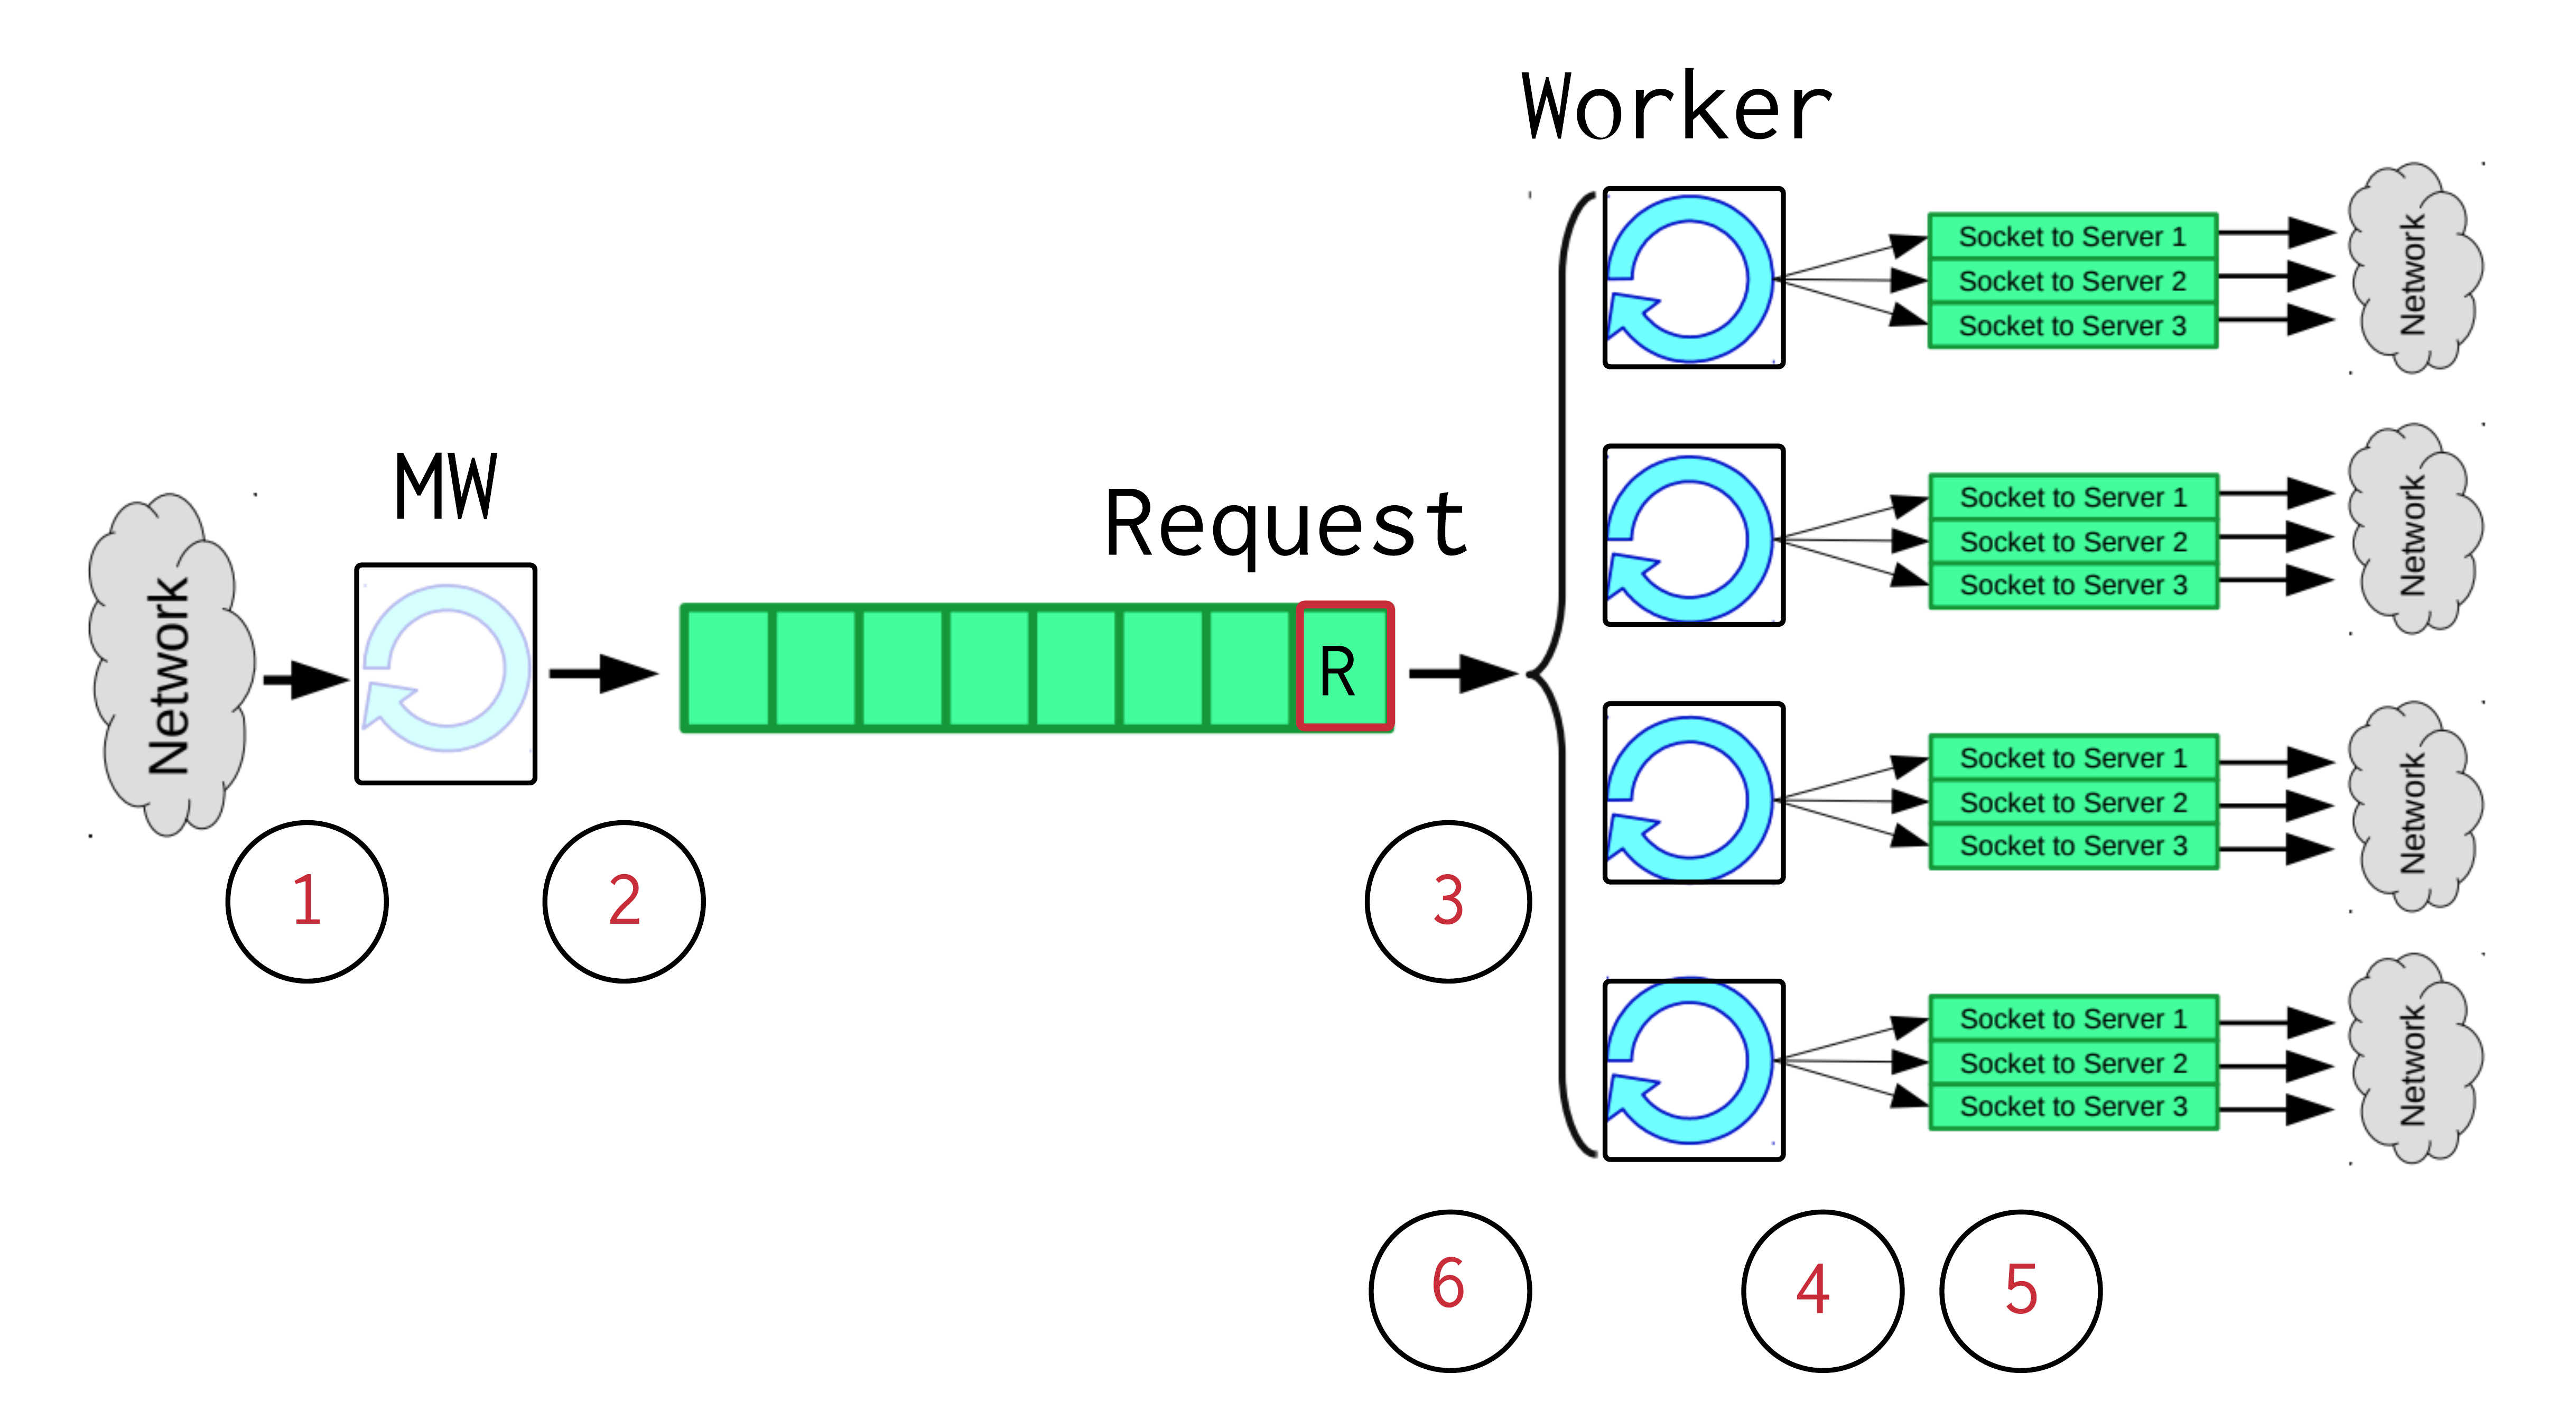
\includegraphics[width=0.8\textwidth]{figures/architecture.png}
    \label{fig:architecture}
    \caption{Middleware architecture.}
\end{figure}

The Middleware is instrumented at six points (shown in Fig.\ref{fig:architecture}):

\begin{enumerate}
    \item $R_{c}$ - Request created
    \item $R_{e}$ - Request enqueued
    \item $R_{d}$ - Request dequeued
    \item $R_{f}$ - Request forwarded to memcached instances.
    \item $R_{r}$ - Response received from memcached instances.
    \item $R_{a}$ - Request answered to memtier instance.
\end{enumerate}

\subsection{Load Balancing}

In order to guarantee that each server gets the same amount of jobs, each request's key gets hashed to a specific index that identify a memcached instance.\\This is done by method \texttt{getServerFromKey} in \texttt{Worker} class, and further tested in class \texttt{LoadBalancer} of package \texttt{test.java.asl}. Following is the result of a test with 1M random strings and 10 servers: \\\\
\texttt{
    Server 0 got 100047 jobs.\\
    Server 1 got 100172 jobs.\\
    Server 2 got 99590 jobs.\\
    Server 3 got 99714 jobs.\\
    Server 4 got 100506 jobs.\\
    Server 5 got 100081 jobs.\\
    Server 6 got 99962 jobs.\\
    Server 7 got 100221 jobs.\\
    Server 8 got 99809 jobs.\\
    Server 9 got 99898 jobs.\\}

This indeed shows that the distribution is uniform and that each memcached instance receives the same amount of requests as the others.\\\textbf{NOTE:} This is done only for \texttt{GET} and \textit{non-sharded} \texttt{MULTI-GET}s requests, as \texttt{SET}s need to be replicated, and \textit{sharded} \texttt{MULTI-GET}s are splitted across memcached instances. 

\subsection{The system}

There are two main components, the \texttt{MW} and the \texttt{Worker}s. They communicate between each other using a dynamic-sized queue where requests are passed in.

\subsection{The queue}

The queue is designed to grow as much as needed although in practice it can only grow to the number of clients memtier is using. A fixed-sized queue may have done the job as well, but having a dynamic-sized one has less impact on the memory usage.

\subsection{Non-blocking IO}

The Middleware communicate both with the clients and the memcached instances via the \texttt{java.NIO.SocketChannel}'s library. In \texttt{MW}'s constructor \texttt{Worker}'s are instantiated and started. Each \texttt{Worker}, connects to the memcached instances in a non-blocking fashion.

\subsection{Request Protocol}

Each request is assumed to be well-formed, and only the first character is checked in order to determine the request type. As a request may be sent into multiple chunks, it is essential to read it without losing any byte. Thisis done by saving the partial content of the \texttt{ByteBuffer} the \texttt{SocketChannel} has written to, into a \texttt{ByteArrayOutputStream}. A request is assumed to be completed when the last bytes are equals to\texttt{"\textbackslash{}r\textbackslash{}n"}. The same assumption is done for responses from the memcached instances, by checking \texttt{"STORED\textbackslash{}r\textbackslash{}n"} or \texttt{"END\textbackslash{}r\textbackslash{}n"}.

\subsection{Handling incoming connections}

The Middleware listens for incoming connections by memtier clients. This is achieved by using the \texttt{java.NIO} package that allows non-blocking IO operations on multiple channels. A \texttt{Selector} monitors channels for changes and signal them in a \texttt{SelectionKey} object, which contains a set of keys registered with the channel. \\Whenever a \texttt{SelectionKey}'s interest is set on \texttt{ACCEPT}, a \texttt{SocketChannel} connection can be established between the client issuing the request and the Middleware. After that, the interest of the \texttt{SelectionKey} is set to \texttt{READ}, waiting for data from the client.

\subsection{Handling incoming requests}

When the \texttt{SelectionKey}'s interest is set to \texttt{READ}, data is read from the \texttt{SocketChannel}. From this moment the Middleware starts recording the \texttt{responseTime} of the request (Point 1 in Fig.\ref{fig:architecture}). When the whole request has been read, it gets enqueued to a \texttt{BlockingQueue}, its \texttt{queueWaitingTime} is started (Point 2 in Fig.\ref{fig:architecture}), and the \texttt{SelectionKey}'s interest is set to \texttt{WRITE}.

\subsection{Forwarding requests}

When a new request is ready to be processed by a \texttt{Worker}, before sending it to the memcached instances, some operations take place (shown in Fig.\ref{fig:dequeue}):

\begin{itemize}
    \item The request's \texttt{queueWaitingTime} is stopped (Point 3 in Fig.\ref{fig:architecture}).
    \item The request gets copied into a \texttt{pendingRequest} object.
    \item Based on its type, a \texttt{multiRequest} object gets created.
\end{itemize}

Then, when the first entry of the \texttt{multiRequest} object gets sent, the \texttt{pendingRequest}'s \texttt{serviceTime} is started (Point 4 in Fig.\ref{fig:architecture}).

\begin{figure}[h]
    \centering
    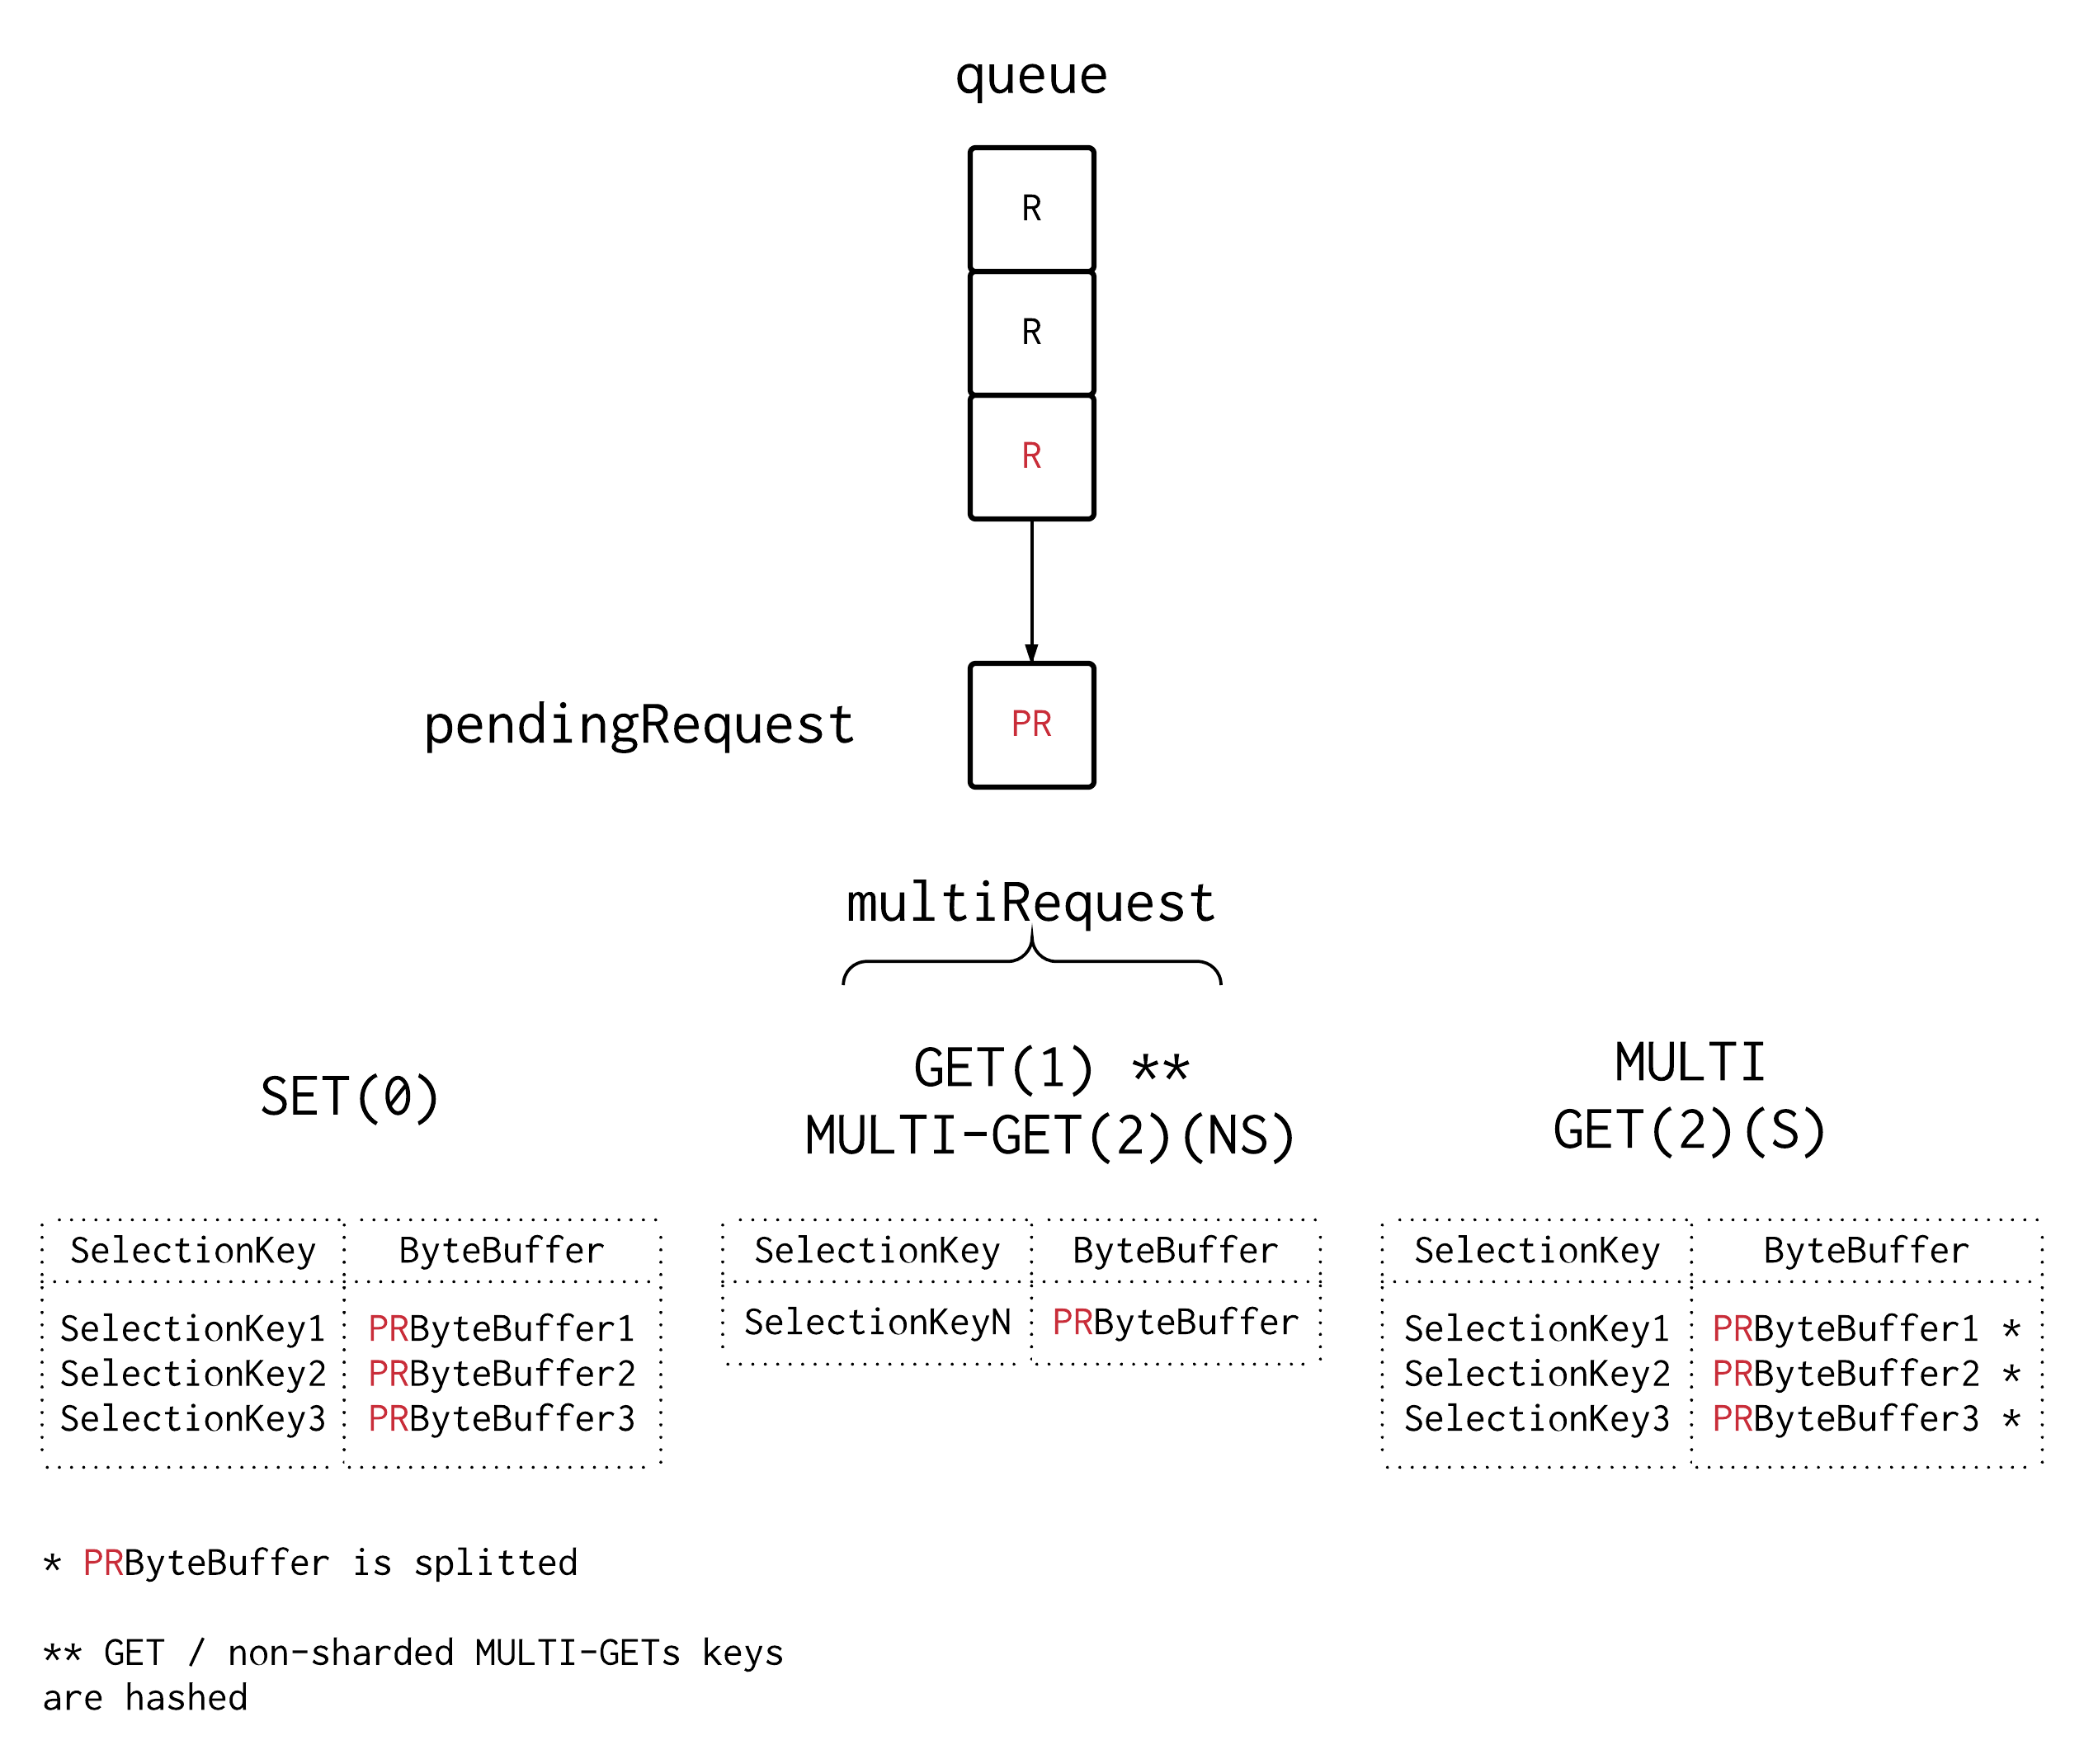
\includegraphics[width=0.9\textwidth]{figures/dequeue.png}
    \label{fig:dequeue}
    \caption{\texttt{loadRequest()} behavior.}
\end{figure}

\subsection{Handling responses}
\label{sec:responses}

When handling an incoming response each \texttt{Worker} does the following:

\begin{itemize}
    \item Checks if the response is completed
    \item Increments a counter of the number of responses received, and compares it with the size of the \texttt{multiRequest} object created for that \texttt{pendingRequest} (expected number of responses).
    \item Then, in case it has received the expected number of responses:
        \begin{itemize}
            \item Stops the \texttt{pendingRequest}'s \texttt{serviceTime} (Point 5 in Fig.\ref{fig:architecture}).
            \item Creates a \texttt{Statistic} object that wraps \texttt{pendingRequest} measures.
            \item Answers back to the client that issued the request.
            \item Stops the \texttt{pendingRequest}s \texttt{responseTime} (Point 6 in Fig.\ref{fig:architecture}).
        \end{itemize}
\end{itemize}        

\subsection{Statistics}
\label{sec:1.10}

As already pointed out in \ref{sec:responses}, each \texttt{Worker} collects the following statistics:

\begin{itemize}
    \item The current system's time (\texttt{ns}).
    \item The time the request spent in the queue (\texttt{ns}).
    \item The time elapsed between forwarding the first \texttt{multiRequest} and the last response (\texttt{ns}).
    \item The time elapsed between reading the request from the client and the last response (\texttt{ns}).
    \item The current queue size.
    \item The number of misses of the request.
    \item The number of keys in the request.
\end{itemize}

\textbf{NOTE:} All the time-related statistics are then converted in milliseconds (\texttt{ms}) when writing them to the logs.

\section{Baseline without Middleware (75 pts)}

In these experiments we study the performance characteristics of the memtier clients and memcached servers.

\subsection{One Server}
\label{sec:2.1}

In this, and in each of the following sections, the number of virtual clients is intended to be the total number of clients in the system, if otherwise, it is emphasized the phrase \textit{per thread}.
Bottleneck analysis, and throughput/response time comparsions are shown in each \textit{Explanation} section of each experiment, rather than in the Summary.
The focus on the latter is in presenting how the maximum throughput configurations are determined.

\subsubsection{Experiment Setting}

There are 3 machines that generate write-only and read-only workloads. Each machine runs a single memtier instance with 2 threads, and from a minimum of 1, to 64 virtual clients \textit{per thread} (see table below).
The number of virtual clients is the only (tunable) parameter in this setting; it is expected that by raising it, both throughput and response time should grow respectively. The reason behind it is that by raising the number of clients, the server  will spend less "idle/free time" between each successive request.
The clients machines are connected to a server machine running a single, one-threaded, memcached instance. Each experiment runs for 70 seconds (measures take into account both warm-up and cool-down phases, excluding 10 secs), and is repeated for 3 times under the same exact conditions.
By running this benchmark, we hope to find how much load can a single memcached instance sustain.

\begin{center}
	\scriptsize{
		\begin{tabular}{|l|c|}
			\hline Number of servers                & 1                        \\ 
			\hline Number of client machines        & 3                        \\ 
			\hline Instances of memtier per machine & 1                        \\ 
			\hline Threads per memtier instance     & 2                        \\
			\hline Virtual clients per thread       & [1, 4, 8, 16, 24, 32, 40, 48, 64]\\ 
			\hline Workload                         & Write-only and Read-only \\
			\hline Multi-Get behavior               & N/A                      \\
			\hline Multi-Get size                   & N/A                      \\
			\hline Number of middlewares            & N/A                      \\
			\hline Worker threads per middleware    & N/A                      \\
            \hline Repetitions                      & 3 (70 secs, effective 60 secs) \\ 
            \hline Log Files Path                   & \texttt{experiments/baseline\_no\_mw\_1\_server/} \\
            \hline Processed Files Path             & \texttt{experiments/baseline\_no\_mw\_1\_server/out/memtier\_data.csv}\\
            \hline
		\end{tabular}
	} 
\end{center}

\subsubsection{Explanation}

The following plot shows how throughput and reponse time behave when increasing the number of virtual clients.
The number of virtual clients on the \texttt{x-axis} of each plot represents the total number of clients in the system, e.g. the first tick at \texttt{VC=6} is the result of \texttt{1} virtual client per thread multiplied by the number of threads (\texttt{2}), instances(\texttt{1}), and client machines(\texttt{3}).
For each quantity we plot the average measured value of the 3 repetitions, and the standard deviation from the mean as a confidence measure.
Additionally as a sanity check, we plot the \textit{Interactive Law} as a dotted line in the troughput plots.
In this case it is computed as the invers of the measured response time multiplied by the total number of virtual clients.
The throughput shown below is the sum of the throughputs of each memtier instance of each client, while the response time is the average response time of each client's machine. 

\subsubsection*{Read-Only}

Consider the throughput below: we can see pretty clearly that, for the whole virtual clients range, apart from \texttt{VCs=6}, (in which the memcached server is still \textbf{under-saturated}), it essentially remains constant at $\approx 3000$ops/s. Suprisingly, increasing the number of virtual clients doesn't affect the throughput at all; the server is indeed saturated after 6 virtual clients. Although we have extended the range of virtual clients per thread to 64, we still cannot observe over-saturation of the server.\\
The same exact behavior can be double checked by looking at the response time plot. It grows almost linearly, confirming the fact that the server is saturated.\\ As for now, (without additional information both on the arrival rate of requests and the service rate at which they get processed), we cannot determine the bottleneck of the sytem. Either outbound load is limited by the client's bandwidth, or the server's peak performance in reading is 3k ops/s. In Section~\ref{sec:2.2} we investigate how much workload a client machine can generate, that is the missing piece of the puzzle to conclude the bottleneck analysis.

\begin{figure}[!h]
  \centering
  \caption{Plots for baseline with one server (read-only)}
  \label{fig:baseline_no_mw_1_server_ro}
  \makebox[\textwidth]{
    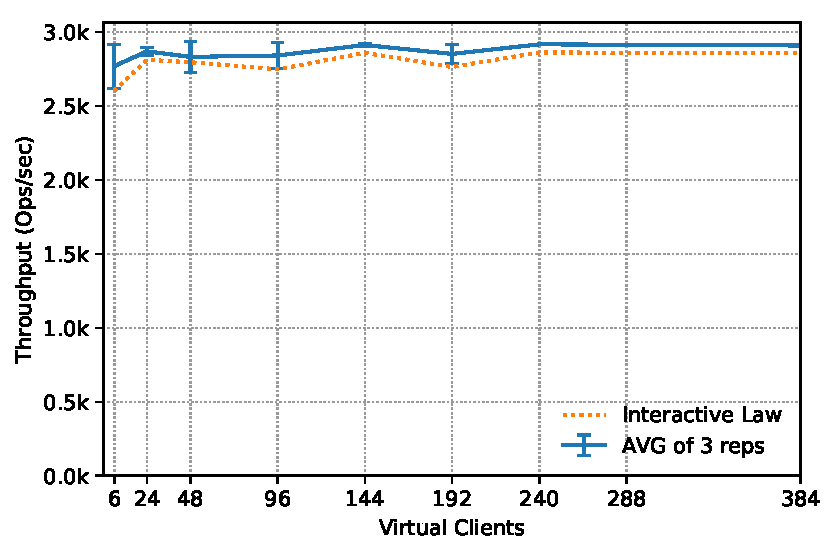
\includegraphics[width=0.6\textwidth]{figures/baseline_no_mw_1_server/tp_memtier_read_only.pdf}
    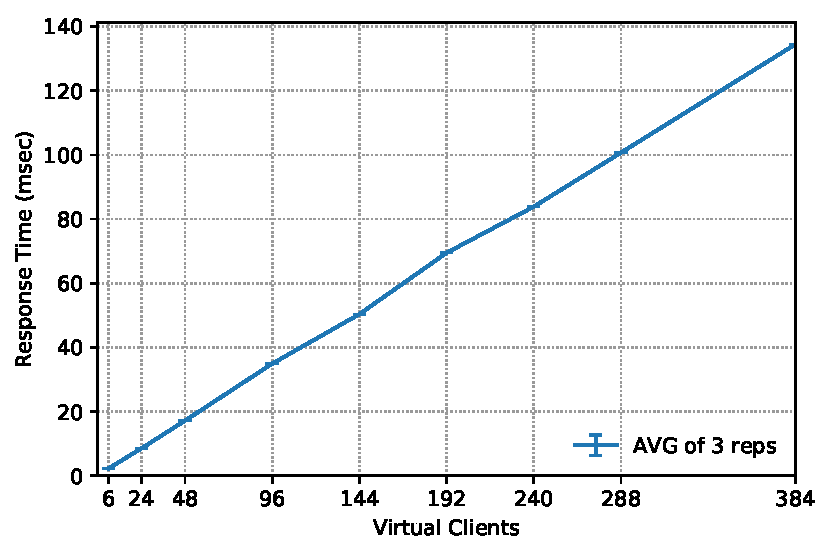
\includegraphics[width=0.6\textwidth]{figures/baseline_no_mw_1_server/rt_memtier_read_only.pdf}
  }
\end{figure}

\subsubsection*{Write-Only}

When testing for write-only workloads we observe a completely different behavior with respect to what seen above. Here the throughput follow our initial assumption and grows as the number of virtual clients increases. We can see that at \texttt{VCs=240} we reach saturation. We can explain the fact that we reach saturation at a much higher number of VCs compared to the read-only workload, simply because the service rate at which the server process write-only requests, is higher than when reading. This is investigated and further confirmed when measuring service time for different workloads inside the middleware in Section ~\ref{sec:3.1}.
With no surprise, the response time plot reflects the measured throughput: we have an initial under-saturated phase until \texttt{VCs=240}, for which the rate $\dfrac{r_t}{\texttt{VC}}$ monotonically decreases.
After that point, the rate stays almost constant, suggesting a flattening:\\\\
$\dfrac{2.5}{24}= \approx 0.1$\\\\
$\dfrac{4}{48}= \approx 0.08$\\\\
$\dfrac{6}{96}= \approx 0.06$\\\\
$\dfrac{12}{192}= \approx 0.06$\\\\
$\dfrac{14}{240}= \approx 0.058$\\\\
$\dfrac{22}{384}= \approx 0.057$\\\\
In addition, by looking at the interactive law, we can observe that it follows the throughput line precisely, concluding the analysis for the experiment.

\begin{figure}[!h]
  \centering
  \caption{Plots for baseline with one server (write-only)}
  \label{fig:baseline_no_mw_1_server_wo}
  \makebox[\textwidth]{
    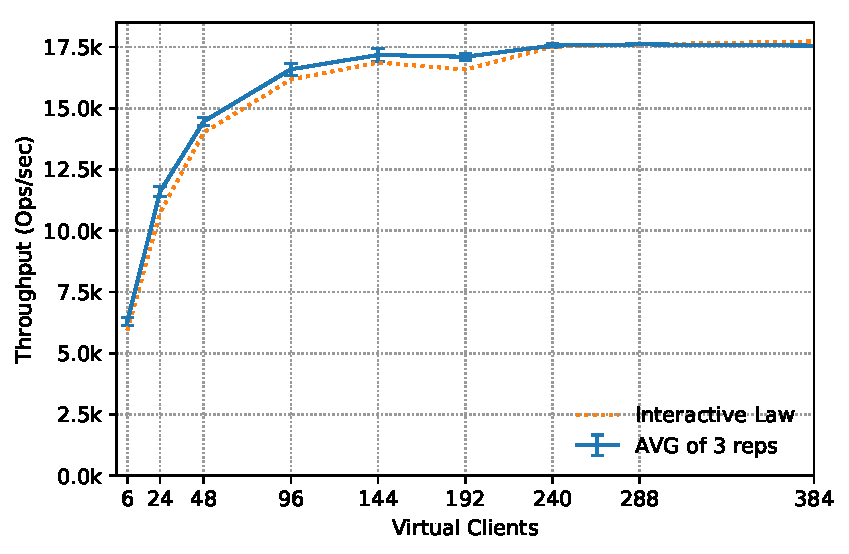
\includegraphics[width=0.6\textwidth]{figures/baseline_no_mw_1_server/tp_memtier_write_only.pdf}
    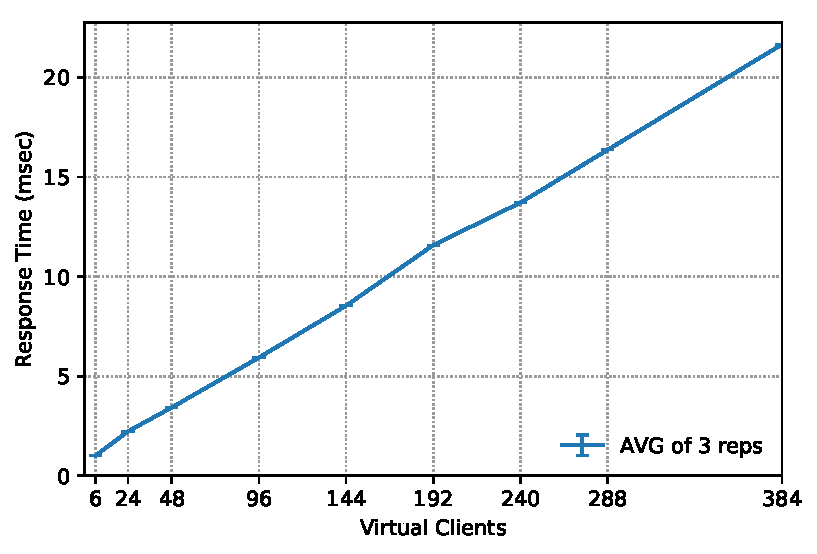
\includegraphics[width=0.58\textwidth]{figures/baseline_no_mw_1_server/rt_memtier_write_only.pdf}
  }
\end{figure}

\subsection{Two Servers}
\label{sec:2.2}

\subsubsection{Experiment Setting}

There is a single client machine that generates write-only and read-only workloads. The machine runs two different memtier instances with 1 thread, and from a minimum of 1, to 32 virtual clients (see table below).
The number of virtual clients is again, the only (tunable) parameter in this setting; it is expected that by raising it, both throughput and response time should grow accordingly. We connect each client's instance to 2 different server machines running a single, one-threaded, memcached instance. The same exact conditions on the number of repetions, duration and measurement stated before still hold. By running this benchmark, we hope to find how much load can a single memtier client produce before saturation.

\begin{center}
	\scriptsize{
		\begin{tabular}{|l|c|}
			\hline Number of servers                & 2                        \\ 
			\hline Number of client machines        & 1                        \\ 
			\hline Instances of memtier per machine & 2                        \\ 
			\hline Threads per memtier instance     & 1                        \\
            \hline Virtual clients per thread       & [1, 4, 8, 16, 24, 32]    \\ 
			\hline Workload                         & Write-only and Read-only \\
			\hline Multi-Get behavior               & N/A                      \\
			\hline Multi-Get size                   & N/A                      \\
			\hline Number of middlewares            & N/A                      \\
			\hline Worker threads per middleware    & N/A                      \\
            \hline Repetitions                      & 3 (70 secs, effective 60 secs) \\ 
            \hline Log Files Path                   & \texttt{experiments/baseline\_no\_mw\_2\_server/} \\
            \hline Processed Files Path             & \texttt{experiments/baseline\_no\_mw\_2\_server/out/memtier\_data.csv}\\
			\hline 
		\end{tabular}
	} 
\end{center}

\subsubsection{Explanation}

Once again we plot both throughput and response time as a function of the total number of clients. It is interesting to note how these quantities are measured. The response time is the mean response time of each memtier instance, for each client machine, for each repetition. The throughput is the sum of the throughputs measured in each instance, summed over the number of client machines, and averaged between each repetition. The error measure introduced is again the standard deviation from the mean value in all repetitions.

\subsubsection*{Read-Only}

The throughput presents an interesting behavior: as before, we observe that it flattens early on, at \texttt{VCs=8}, reaching saturation at $\approx$ 6k $ops/s$. From that point on, the system seems to begin to over-saturate, as the throughput slightly decrases.\\
In Section \ref{sec:2.1} we have 3 clients connected to one server, reaching peak performance at $\approx$ 3k $ops/s$, this suggests that now that we have a single client that can read 6k $ops/s$ from two servers, that the bottleneck when reading is effectively the service rate at which a single memcached instance process incoming requests. The response time, after a sub-linear growth between the first and second virtual clients grows linearly, confirming saturation.

\begin{figure}[!h]
  \centering
  \caption{Plots for baseline with two servers (read-only)}
  \label{fig:baseline_no_mw_2_server_ro}
  \makebox[\textwidth]{
    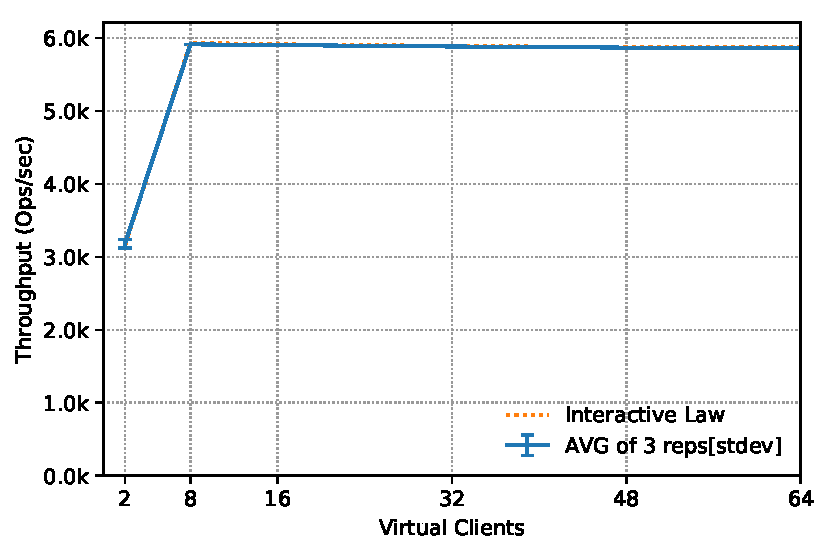
\includegraphics[width=0.6\textwidth]{figures/baseline_no_mw_2_server/tp_memtier_read_only.pdf}
    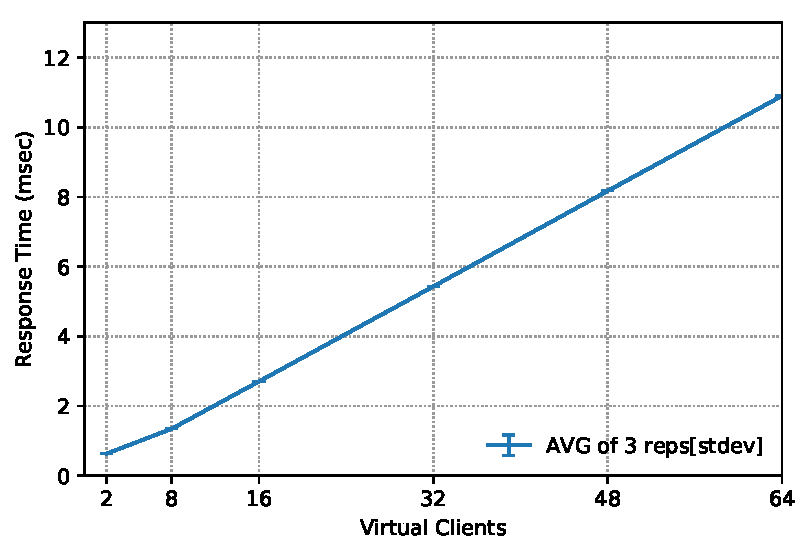
\includegraphics[width=0.6\textwidth]{figures/baseline_no_mw_2_server/rt_memtier_read_only.pdf}
  }
\end{figure}

\subsubsection*{Write-Only}

The throughput is almost identical to the read-only workload. Again a pretty fast flattening at $\num{VCs=8}$. 
Let's compare it with the one in Section \ref{sec:2.1}: there, we have 3 clients writing to a single server, reaching an $\approx$ 18k $ops/s$ peak performance), meaning an approximate throughput per client of 6k $ops/s$.
Now by doubling the number of servers, a single client still produces 6k $ops/s$. 
Thus, we can conclude that the bottleneck is the maximum arrival rate of incoming write-only request from a single client machine, limited at 6k $ops/s$. 

\newpage

\begin{figure}[!h]
  \centering
  \caption{Plots for baseline with two servers (write-only)}
  \label{fig:baseline_no_mw_2_server_wo}
  \makebox[\textwidth]{
    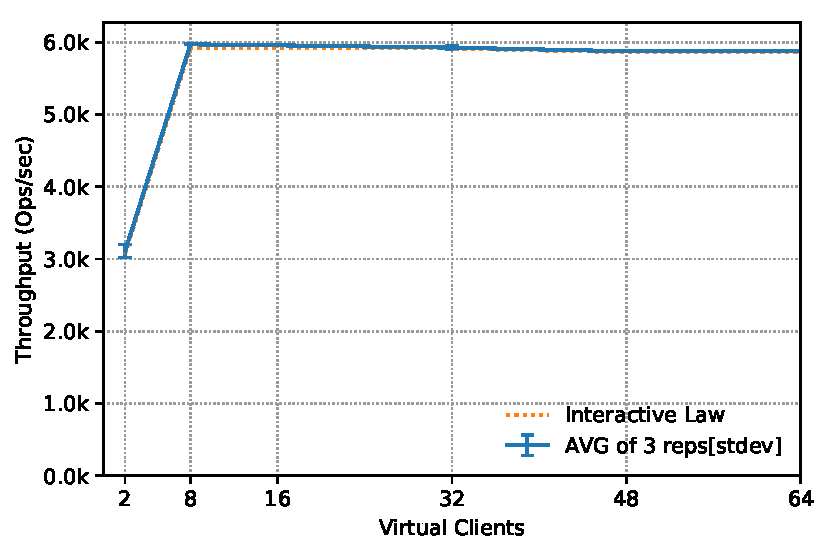
\includegraphics[width=0.6\textwidth]{figures/baseline_no_mw_2_server/tp_memtier_write_only.pdf}
    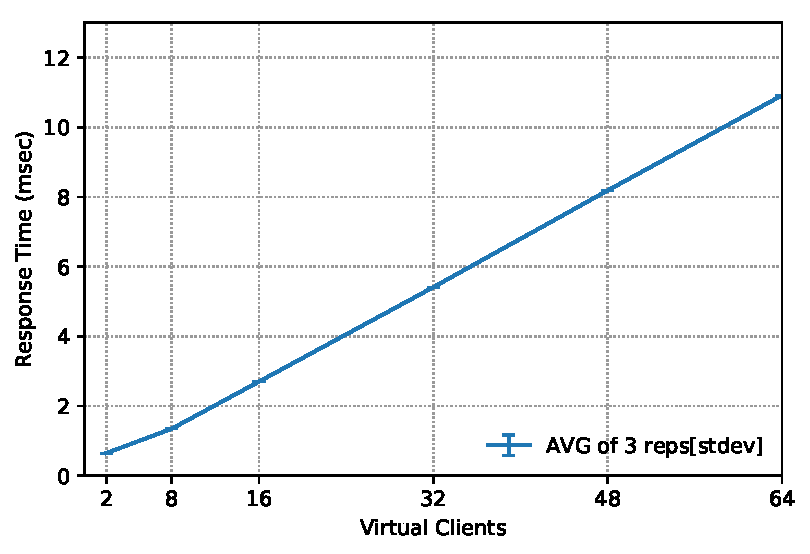
\includegraphics[width=0.6\textwidth]{figures/baseline_no_mw_2_server/rt_memtier_write_only.pdf}
  }
\end{figure}

\subsection{Summary}
\label{sec:2.3}

Following, the maximum throughput of each experiment for both write-only and read-only workload is shown.
In order to determine what is the maximum throughput configuration, we additionally plot the rate of change of the response time over the generated load and pick the configuration from which the rate reaches an horizontal asyntote.
Before that point the response time can grow sub-linearly, even oscillating (in the read-only case). So, we choose the first stable virtual client which rate stays almost flat for the entire range of virtual clients to represent the maximum throughput configuration in our system.

\begin{figure}[!h]
  \centering
  \caption{Plots for baseline with one server (Rate of change of response time over load, left: read-only, right: write-only)}
  \label{fig:baseline_no_mw_1_server_maxtp}
  \makebox[\textwidth]{
    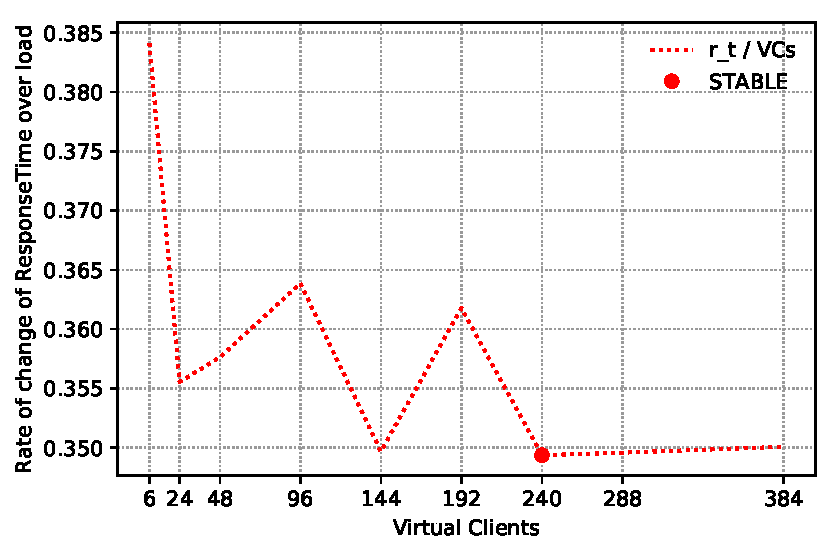
\includegraphics[width=0.6\textwidth]{figures/baseline_no_mw_1_server/maxtp_memtier_read_only.pdf}
    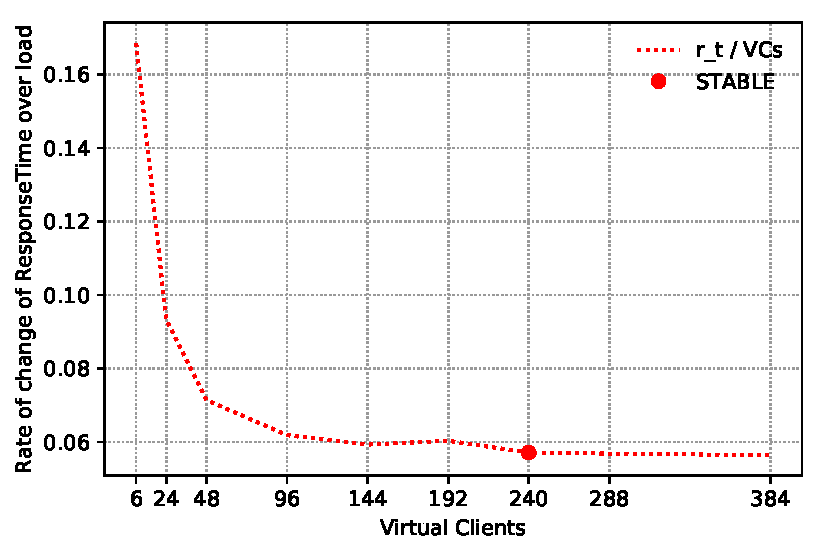
\includegraphics[width=0.6\textwidth]{figures/baseline_no_mw_1_server/maxtp_memtier_write_only.pdf}
  }
\end{figure}

\begin{figure}[!h]
  \centering
  \caption{Plots for baseline with two servers (Rate of change of response time over load, left: read-only, right: write-only)}
  \label{fig:baseline_no_mw_2_server_maxtp}
  \makebox[\textwidth]{
    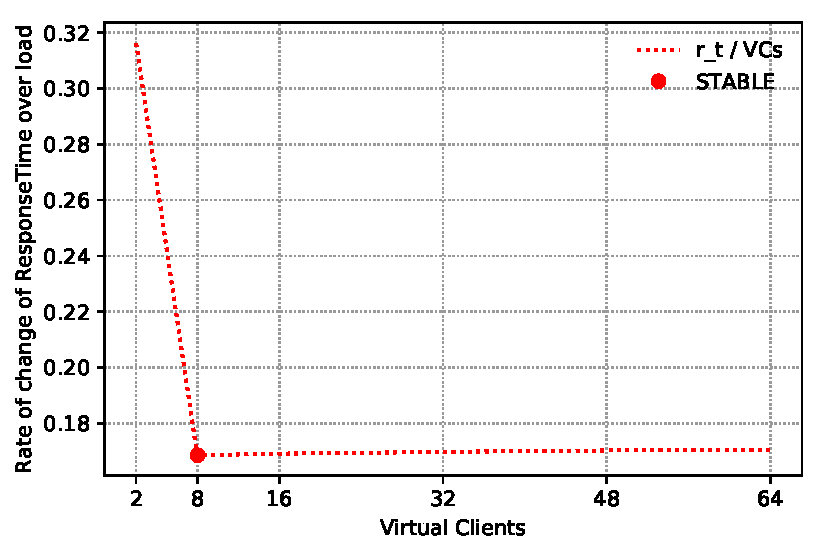
\includegraphics[width=0.6\textwidth]{figures/baseline_no_mw_2_server/maxtp_memtier_read_only.pdf}
    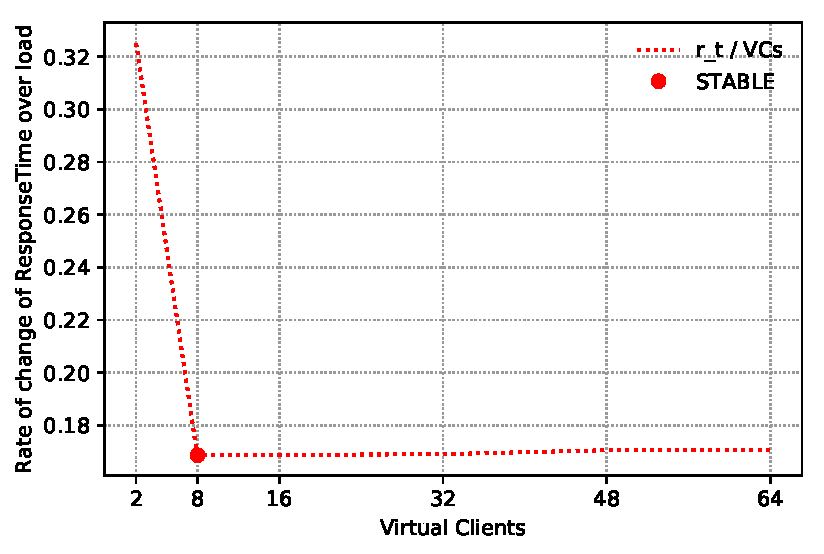
\includegraphics[width=0.6\textwidth]{figures/baseline_no_mw_2_server/maxtp_memtier_write_only.pdf}
  }
\end{figure}

\begin{center}
	{Maximum throughput of different VMs.}
	\begin{tabular}{|l|p{2cm}|p{2cm}|p{4cm}|}
		\hline                        & Read-only workload & Write-only workload & Configuration gives max. throughput  \\ 
        \hline One memcached server   & 2.88k ops/s        & 17.5k ops/s         & 40 VCs per thread (240 total clients)\\ 
        \hline One load generating VM & 5.87k ops/s        & 5.98k ops/s         & 4 VCs per thread (8 total clients)   \\  
		\hline 
	\end{tabular}
\end{center}

When performing write-only operations, each client machine cannot issue more than $\approx$ 6k $ops/s$. Given that the object size is \texttt{4096B}, the maximum throughput achievable is approximately 24 MB/s.
When reading data from the memcached servers, the bottleneck is given by the number of operations a server sends back to the client. Benchmarks indicate that a single memcached machine cannot send more than $\approx$ 3k $ops/s$, or 12 MB/s.

\section{Baseline with Middleware (90 pts)}
\label{sec:3}

In this set of experiments we test the performance of the Middleware/s. 
We measure and display the results both at the client, and inside the middleware, and compare them.
Additionally, in order to gain a better insight on the internal performance breakdown of the middleware, and run analysis on the components, we present the statistics introduced in Section \ref{sec:1.10}.

\subsection{One Middleware}
\label{sec:3.1}

\subsubsection{Experiment Setting}

There are 3 clients machine generating both write-only and read-only workload. Each client machine runs a single memtier instance with 1 thread, and from a minimum of 1, to 64 virtual clients (see table below).
Each client machine is connected to the the middleware, which is connected to a single, one-threaded, memcached machine.
Essentially we are tuning the load the clients produce, and the service rate at which the middleware dispatches request between client and server machines. 

\begin{center}
	\scriptsize{
		\begin{tabular}{|l|c|}
			\hline Number of servers                & 1                        \\ 
			\hline Number of client machines        & 3                        \\ 
			\hline Instances of memtier per machine & 1                        \\ 
			\hline Threads per memtier instance     & 2                        \\
            \hline Virtual clients per thread       & [1, 4, 8, 16, 24, 32, 64]\\ 
			\hline Workload                         & Write-only and Read-only \\
			\hline Multi-Get behavior               & N/A                      \\
			\hline Multi-Get size                   & N/A                      \\
			\hline Number of middlewares            & 1                        \\
			\hline Worker threads per middleware    & [8, 16, 32, 64]                  \\
            \hline Repetitions                      & 3 (70 secs, effective 60 secs) \\ 
            \hline Log Files Path                   & \texttt{experiments/baseline\_mw\_1\_mw/logs} \\
            \hline Processed Files Path             & \texttt{experiments/baseline\_mw\_1\_mw/out/memtier\_data.csv}\\
            \hline
		\end{tabular}
	} 
\end{center}

\subsubsection{Explanation}

We plot throughput and response time as measured at the client and inside the middleware, for an increasing number of both virtual clients and  worker threads.\\
The measurements conducted in the middleware are grouped in five-seconds windows for a total of 14 per experiment ($ 70.0 / 5.0 = 14$). Everytime a request has been processed, and a response has been sent back to the client machines, the measurements for the specific request, and a snapshot of the system components, gets saved and later, processed and logged.\\
Measurements taken inside the middleware, do not include the latency between the client machines and the middleware, so there's a gap between the two, that remains constant and negligible ($\approx 2 ms$).

\subsubsection*{Read-Only}

As in Section~\ref{sec:2.1}, the throughput plot shows a flattening at $\approx$ 3k $op/s$ starting from \texttt{VCs=24}.  The presence of the middleware doesn't seem to affect the performance at all, moreover we cannot spot any differences when changing the number of worker threads inside the middleware. The unique possible explanation, (as we can exclude the fact that the client machines are the bottleneck, from what we have concluded in Section~\ref{sec:2.3}), is again. the fact that a single memcached machine cannot send back more than 3k $ops/s$ of read-only requests.

\begin{figure}[!h]
  \centering
  \caption{Plots for baseline with one Middleware (read-only CLIENT)}
  \label{fig:baseline_mw_1_mw_mt_ro}
  \makebox[\textwidth]{
    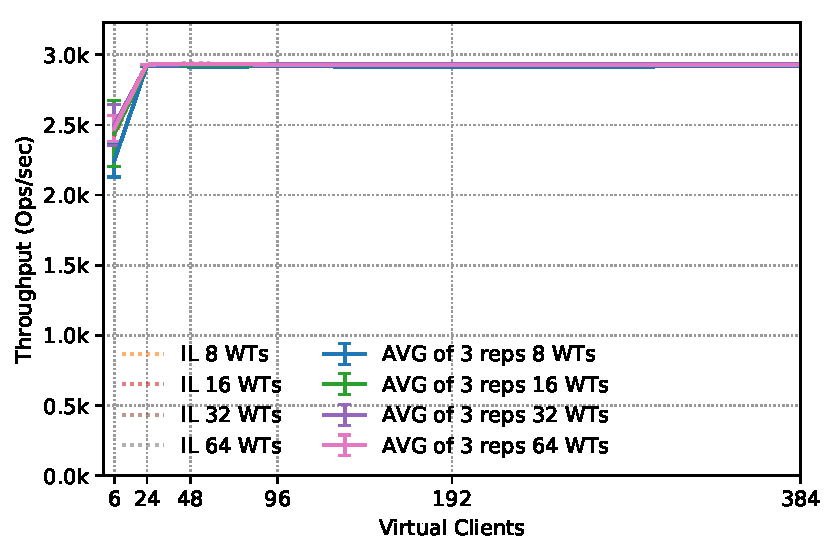
\includegraphics[width=0.6\textwidth]{figures/baseline_mw_1_mw/tp_memtier_read_only.pdf}
    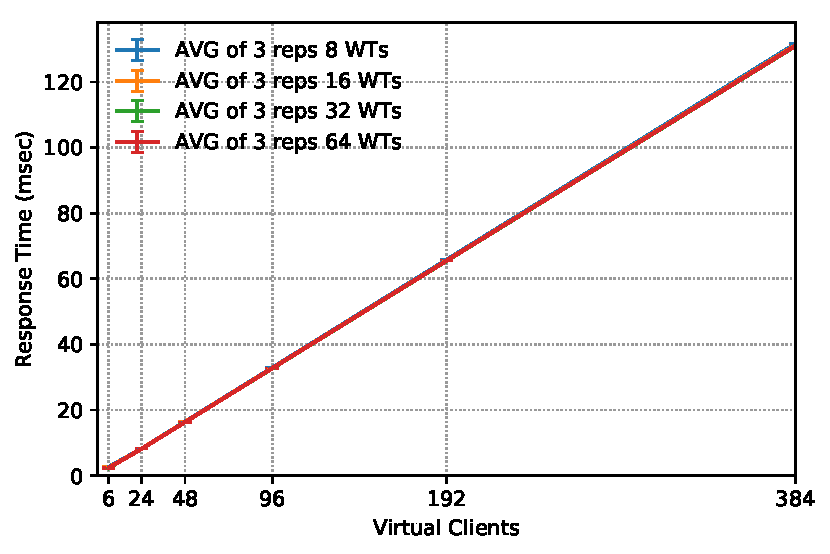
\includegraphics[width=0.6\textwidth]{figures/baseline_mw_1_mw/rt_memtier_read_only.pdf}
  }
\end{figure}

\begin{figure}[!h]
  \centering
    \caption{Plots for baseline with one Middleware (read-only MIDDLEWARE)}
  \label{fig:baseline_mw_1_mw_mw_ro}
  \makebox[\textwidth]{
    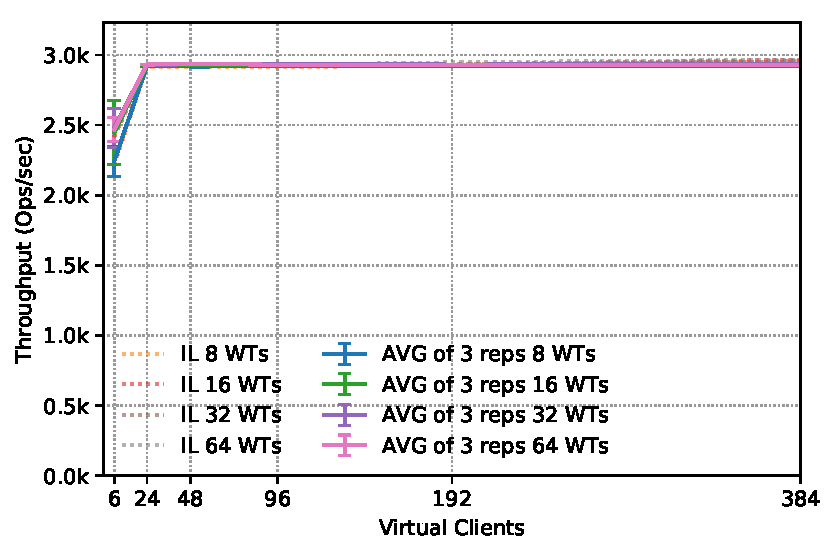
\includegraphics[width=0.6\textwidth]{figures/baseline_mw_1_mw/tp_middleware_read_only.pdf}
    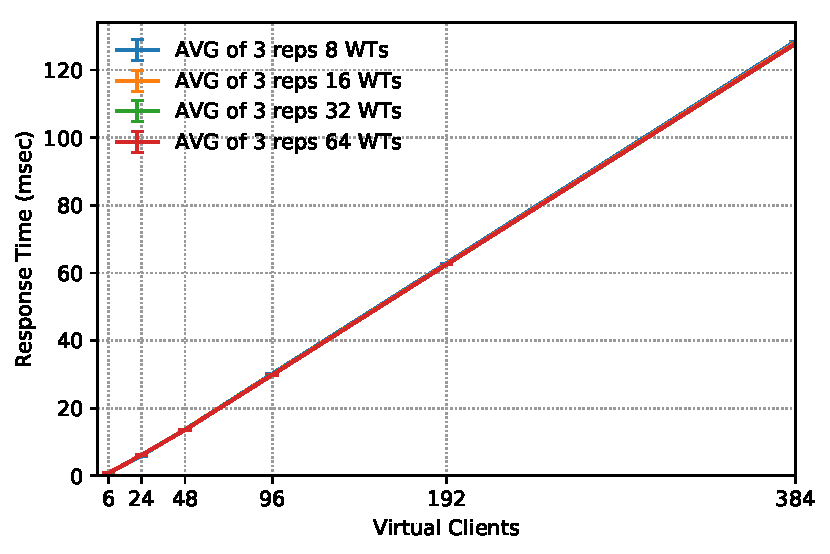
\includegraphics[width=0.6\textwidth]{figures/baseline_mw_1_mw/rt_middleware_read_only.pdf}
  }
\end{figure}

\begin{figure}[!h]
  \centering
    \caption{Plots for baseline with one Middleware, Service Time and Queue Waiting Time (read-only MIDDLEWARE)}
  \label{fig:baseline_mw_1_mw_mw_c_ro}
  \makebox[\textwidth]{
    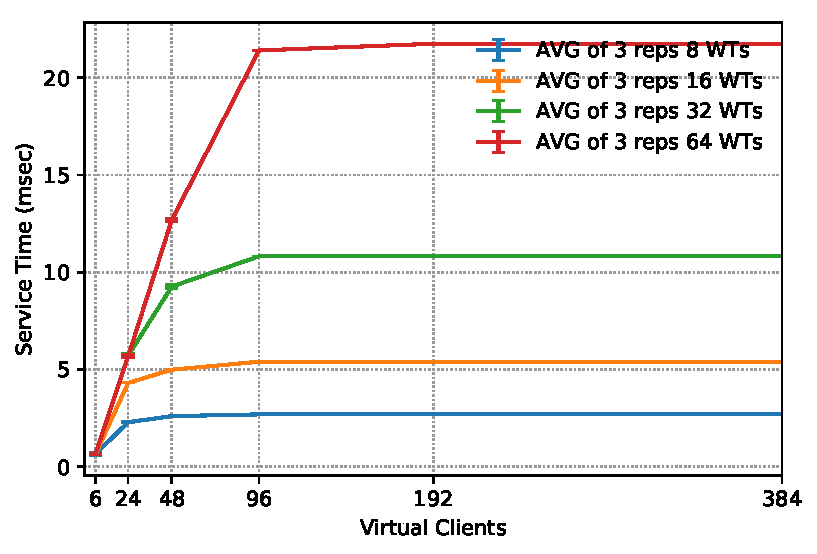
\includegraphics[width=0.6\textwidth]{figures/baseline_mw_1_mw/st_middleware_read_only.pdf}
    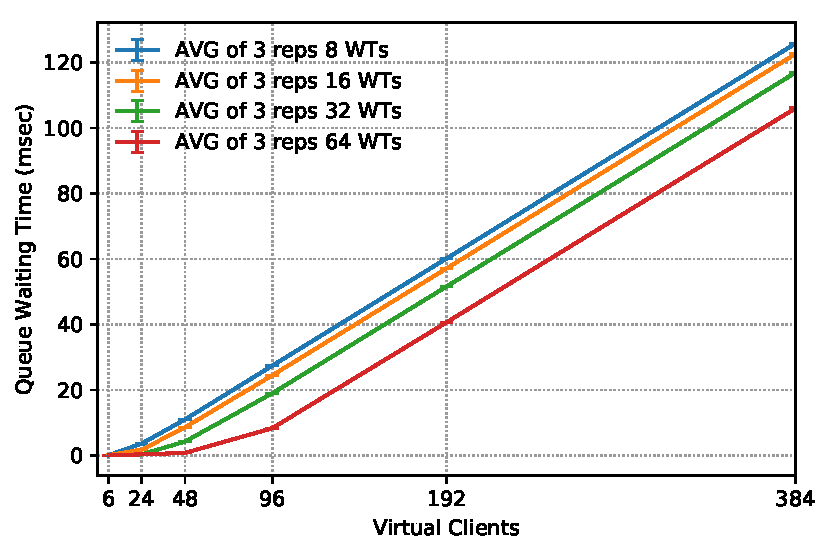
\includegraphics[width=0.6\textwidth]{figures/baseline_mw_1_mw/wt_middleware_read_only.pdf}
  }
\end{figure}

\begin{figure}[!h]
  \centering
    \caption{Plots for baseline with one Middleware (read-only MIDDLEWARE)}
  \label{fig:baseline_mw_1_mw_mw_ro}
  \makebox[\textwidth]{
    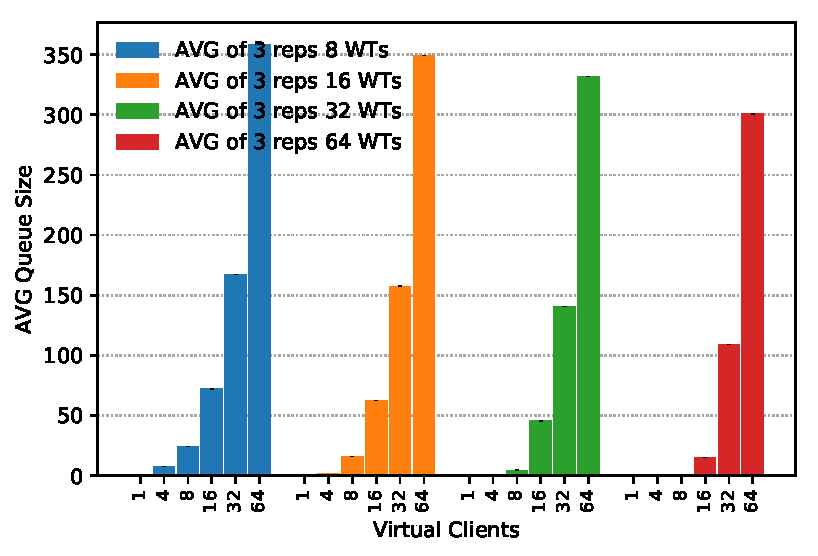
\includegraphics[width=0.6\textwidth]{figures/baseline_mw_1_mw/qs_middleware_read_only.pdf}
  }
\end{figure}

\subsubsection*{Write-Only}

As expected, increasing the number of worker threads in the middleware, results in an increase of the throughput. Even though, for every distinct worker thread configuration, we observe a distinct throughput behavior, there's a common treat that each configuration seems to manifest. In fact we can clearly identify and split the plot in two phases: one that goes from 6 to 192 \texttt{VCs}, and another one, that goes from 192 to 384 \texttt{VCs}. 
In the former (under-saturated phase), the configurations with 16, 32 and 64 workers, behave almost identically (apart from when we reach \texttt{VCs=96}, where we observe a difference of $\approx$ 500-600 $ops/s$).
The latter phase (saturated) shows a much larger difference in performance for different worker threads configurations. We observe a clear distinction between 8 and 16 worker threads, and between 16 and 32, but not as much between 32 and 64 worker threads. 
Comparing this plot to the one in Section~\ref{sec:2.1}, we can cleary see that the presence of the middleware seems to have an impact on the throughput (saturation starts at 12k $ops/s$, before $\approx$ 18k ops/s). The difference is around 30\%.

\begin{figure}[!h]
  \centering
  \caption{Plots for baseline with one Middleware (write-only CLIENT)}
  \label{fig:baseline_mw_1_mw_mt_wo}
  \makebox[\textwidth]{
    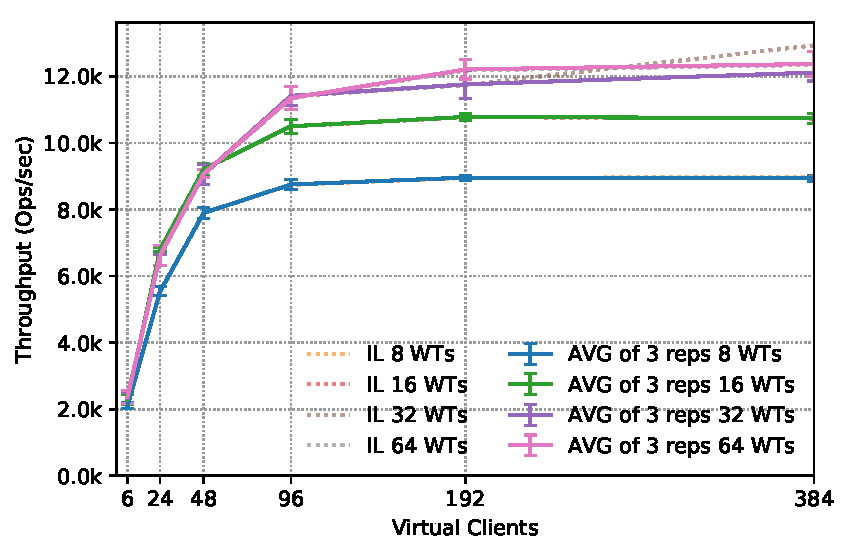
\includegraphics[width=0.6\textwidth]{figures/baseline_mw_1_mw/tp_memtier_write_only.pdf}
    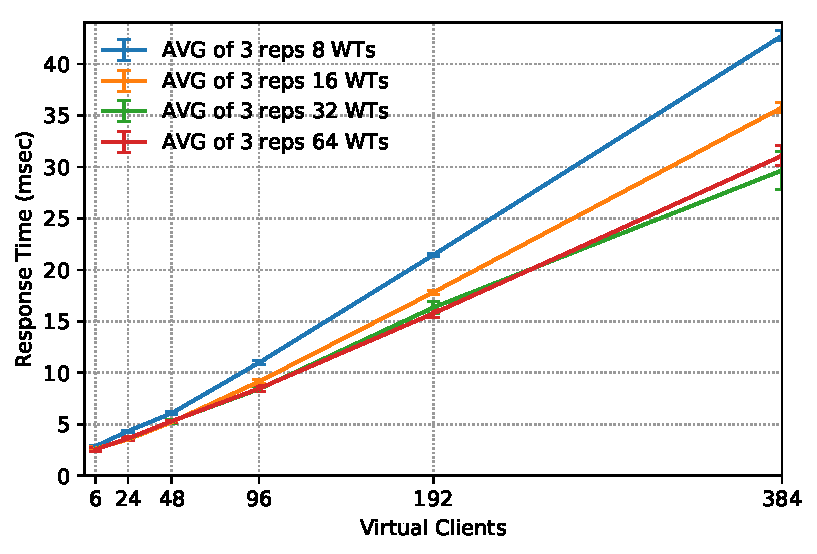
\includegraphics[width=0.6\textwidth]{figures/baseline_mw_1_mw/rt_memtier_write_only.pdf}
  }
\end{figure}

\begin{figure}[!h]
  \centering
  \caption{Plots for baseline with one Middleware (write-only MIDDLEWARE)}
  \label{fig:baseline_mw_1_mw_mw_wo}
  \makebox[\textwidth]{
    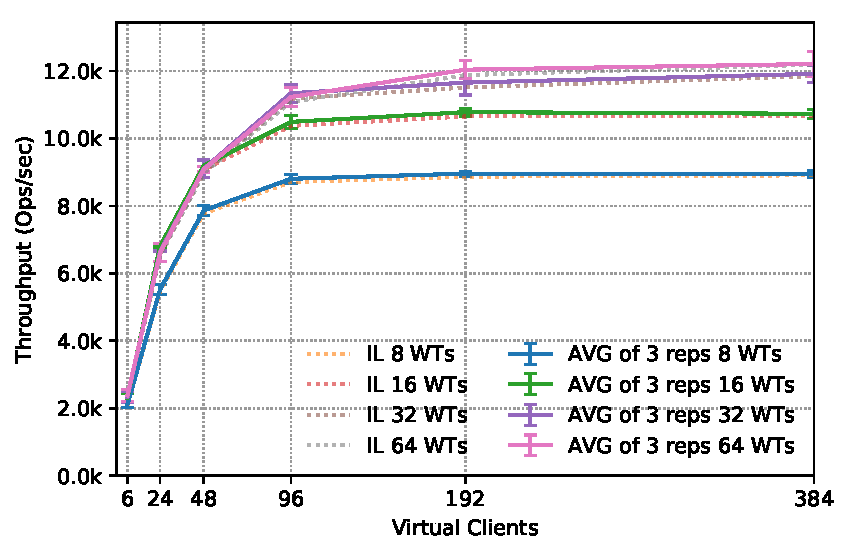
\includegraphics[width=0.6\textwidth]{figures/baseline_mw_1_mw/tp_middleware_write_only.pdf}
    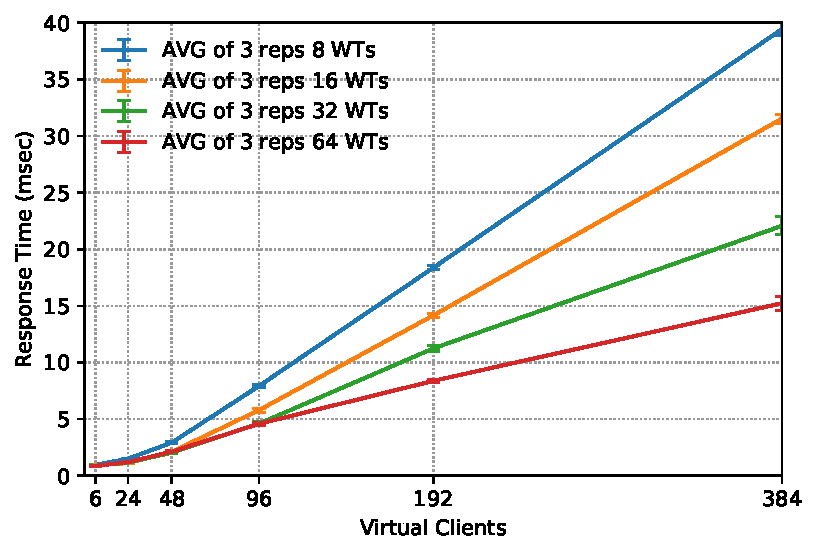
\includegraphics[width=0.6\textwidth]{figures/baseline_mw_1_mw/rt_middleware_write_only.pdf}
  }
\end{figure}

\begin{figure}[!h]
  \centering
  \caption{Plots for baseline with one Middleware, Service Time and Queue Waiting Time (write-only MIDDLEWARE)}
  \label{fig:baseline_mw_1_mw_mw_c_wo}
  \makebox[\textwidth]{
    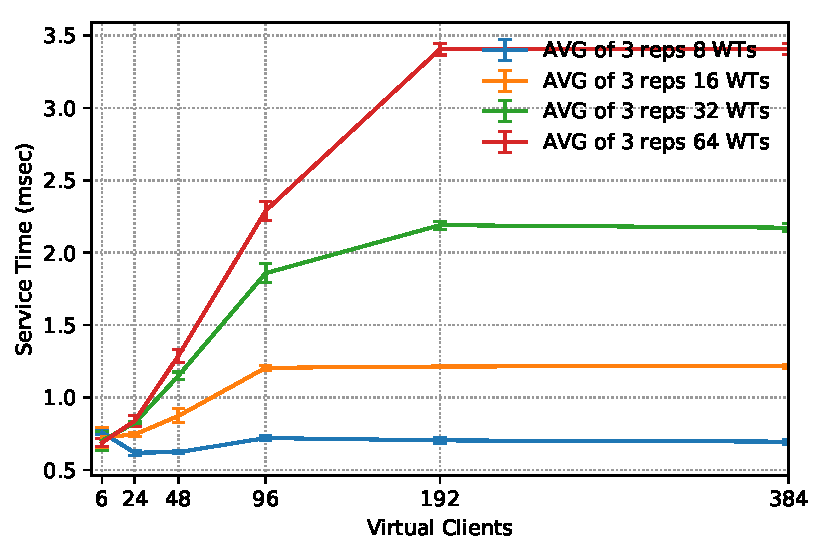
\includegraphics[width=0.6\textwidth]{figures/baseline_mw_1_mw/st_middleware_write_only.pdf}
    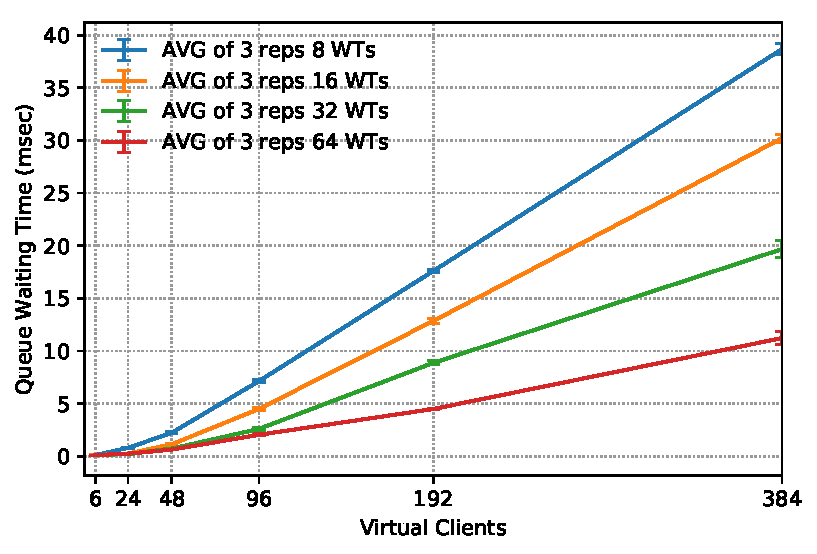
\includegraphics[width=0.6\textwidth]{figures/baseline_mw_1_mw/wt_middleware_write_only.pdf}
  }
\end{figure}

\begin{figure}[!h]
  \centering
    \caption{Plots for baseline with one Middleware, Average Queue Size (write-only MIDDLEWARE)}
  \label{fig:baseline_mw_1_mw_mw_qs_wo}
  \makebox[\textwidth]{
    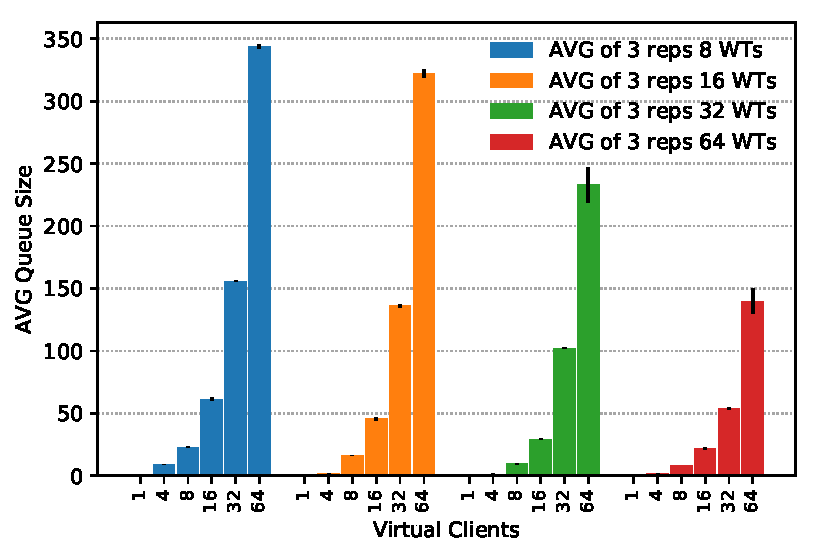
\includegraphics[width=0.6\textwidth]{figures/baseline_mw_1_mw/qs_middleware_write_only.pdf}
  }
\end{figure}


\subsection{Two Middlewares}
\label{sec:3.2}

\subsection{Experiment Setting}

This experiment is similar to the previous one, apart from the fact that here we introduce a new middleware machine.
Again, we have 3 load generating machines that run 2 single-threaded instances of memtier. Each instance connects to a different middleware, which itself, connects to one single-threaded memcached machine. Also in this experiment, we change the number of worker threads inside the middlewares to see how that impacts the overall performance.

\begin{center}
	\scriptsize{
		\begin{tabular}{|l|c|}
			\hline Number of servers                & 1                        \\ 
			\hline Number of client machines        & 3                        \\ 
			\hline Instances of memtier per machine & 2                        \\ 
			\hline Threads per memtier instance     & 1                        \\
			\hline Virtual clients per thread       & [1, 4, 8, 16, 32, 64]                  \\ 
			\hline Workload                         & Write-only and Read-only \\
			\hline Multi-Get behavior               & N/A                      \\
			\hline Multi-Get size                   & N/A                      \\
			\hline Number of middlewares            & 2                        \\
			\hline Worker threads per middleware    & [8, 16, 32, 64]                  \\
            \hline Repetitions                      & 3 (70 secs, effective 60 secs) \\ 
            \hline Log Files Path                   & \texttt{experiments/baseline\_mw\_2\_mw/logs} \\
            \hline Processed Files Path             & \texttt{experiments/baseline\_mw\_2\_mw/out/memtier\_data.csv}\\
            \hline
		\end{tabular}
	} 
\end{center}

\subsubsection{Explanation}

We plot throughput and response time as measured at the client and inside the middleware, for an increasing number of both virtual clients and  worker threads.\\
The same conditions on the measurements presented in Section~\ref{sec:3.1}, still hold. Here, we need to take into account the fact that we have an additional middleware, thus any measure done in one middleware needs to be properly treated. By this we mean that depending on the measurement that we are analyzing, we might either take the  average between the two Middlewares (e.g. response time, service time, and queue waiting time), or some over (e.g. throughput).
It is relevant to mention how such measures are computed, because, as we will see, they might be source for minor imprecisions in the plots.

\subsubsection*{Read-Only}

The client throughput seems to reflect the behavior seen in Section~\ref{sec:2.1}, showing a flattening at $\approx$ 3k $op/s$ starting from \texttt{VCs=24}. If we look at the middleware plot, we still observe the same behavior, this time though, we observe a difference between 8 and 16 worker threads, and between them and 32 and 64. The configurations with 8 and 16 worker threads, exceed 3k $ops/s$. Now, we know that that's not possible, the reason for that is again that when reading we are limited by the memcached server at 3k $ops/s$. This is due to both the fact that time measurements inside the middleware are smaller than the one measured by the clients, and to the systematic error introduced when taking the average between the two.
The difference between the clients and the middlewares plots can be spotted also by looking at their response time/load. In the one measured by the clients, every worker thread configuration is collinear, whereas in the middleware, we have distinct lines for 8 and 16 workers: indeed their value is lower, causing the throughput to grow and pass the 3k $ops/s$ barrier.

\begin{figure}[!h]
  \centering
  \caption{Plots for baseline with two Middlewares (read-only CLIENT)}
  \label{fig:baseline_mw_2_mw_mt_ro}
  \makebox[\textwidth]{
    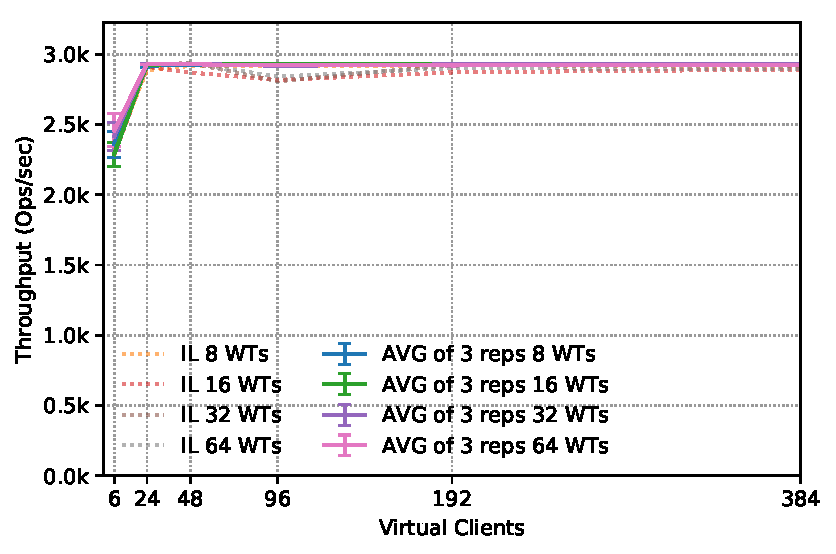
\includegraphics[width=0.6\textwidth]{figures/baseline_mw_2_mw/tp_memtier_read_only.pdf}
    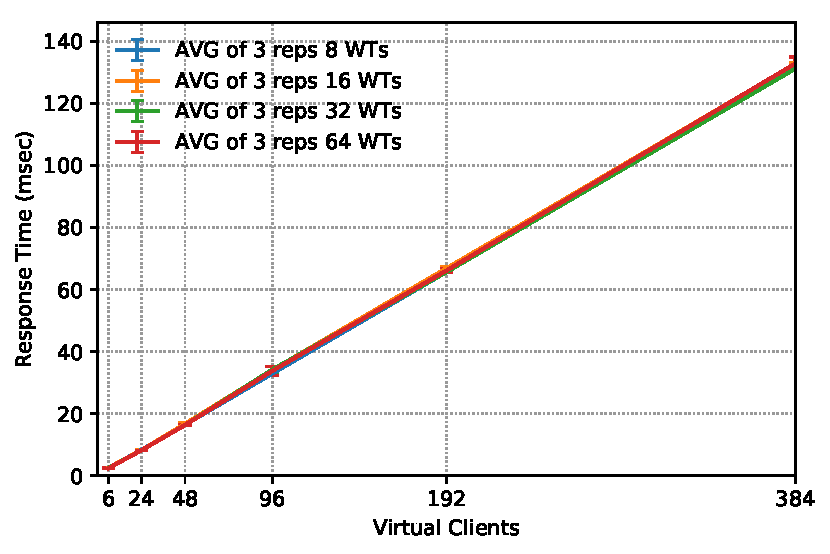
\includegraphics[width=0.6\textwidth]{figures/baseline_mw_2_mw/rt_memtier_read_only.pdf}
  }
\end{figure}

\begin{figure}[!h]
  \centering
    \caption{Plots for baseline with two Middlewares (read-only MIDDLEWARE)}
  \label{fig:baseline_mw_2_mw_mw_ro}
  \makebox[\textwidth]{
    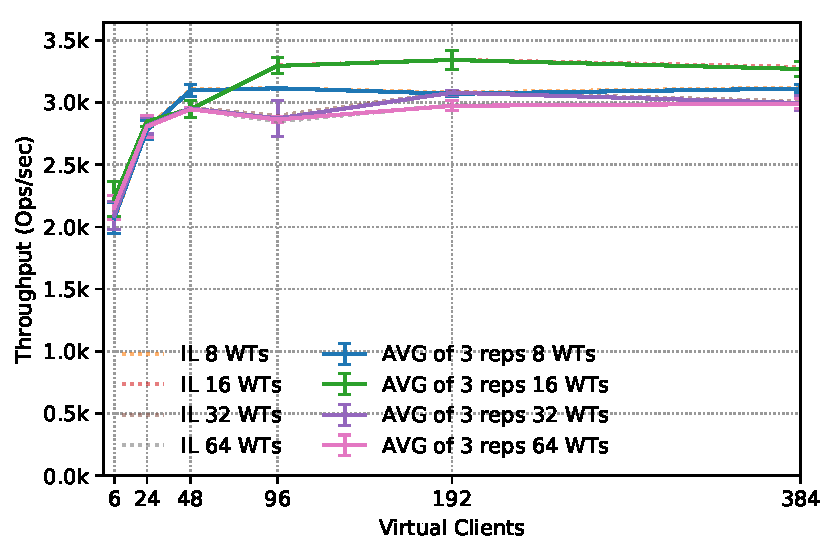
\includegraphics[width=0.6\textwidth]{figures/baseline_mw_2_mw/tp_middleware_read_only.pdf}
    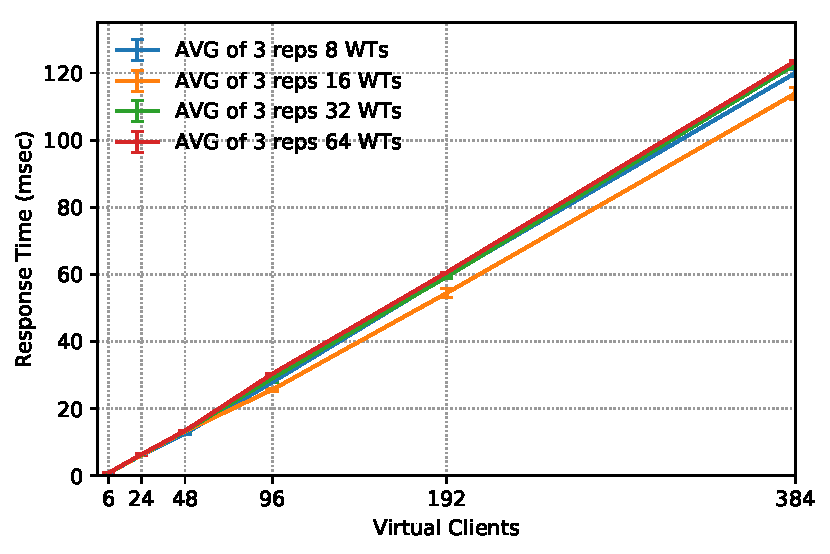
\includegraphics[width=0.6\textwidth]{figures/baseline_mw_2_mw/rt_middleware_read_only.pdf}
  }
\end{figure}

\begin{figure}[!h]
  \centering
    \caption{Plots for baseline with two Middlewares, Service Time and Queue Waiting Time (read-only MIDDLEWARE)}
  \label{fig:baseline_mw_2_mw_mw_c_ro}
  \makebox[\textwidth]{
    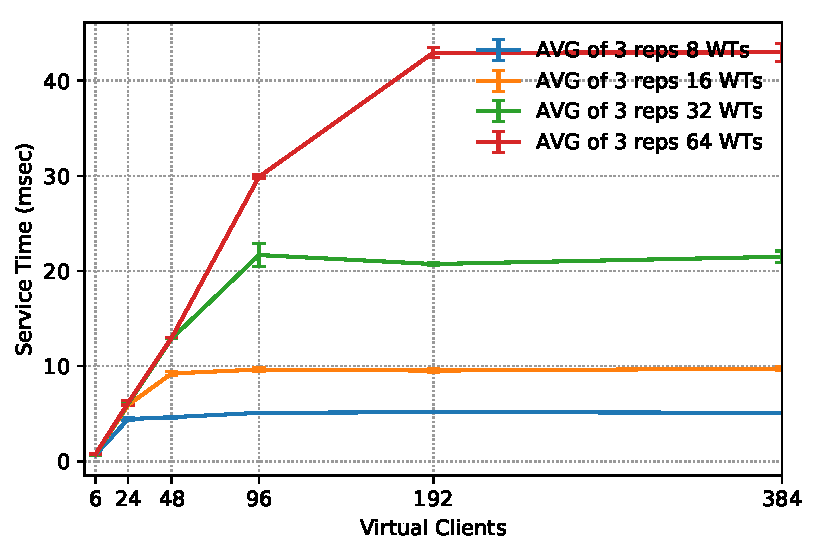
\includegraphics[width=0.6\textwidth]{figures/baseline_mw_2_mw/st_middleware_read_only.pdf}
    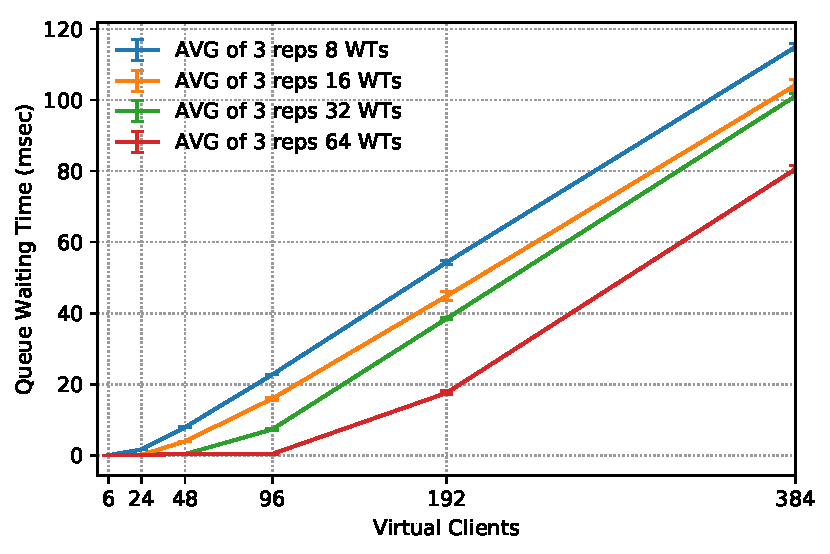
\includegraphics[width=0.6\textwidth]{figures/baseline_mw_2_mw/wt_middleware_read_only.pdf}
  }
\end{figure}

\begin{figure}[!h]
  \centering
    \caption{Plots for baseline with two Middlewares (read-only MIDDLEWARE)}
  \label{fig:baseline_mw_2_mw_mw_ro}
  \makebox[\textwidth]{
    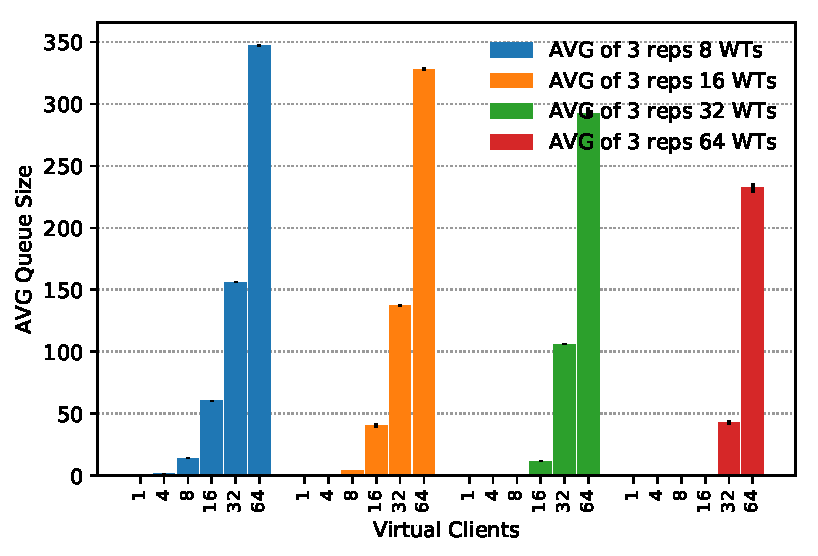
\includegraphics[width=0.6\textwidth]{figures/baseline_mw_2_mw/qs_middleware_read_only.pdf}
  }
\end{figure}

\subsubsection*{Write-Only}

As in the read-only case, we reach the same maximum performance presented in Section \ref{sec:2.1}. It's the configuration with 64 worker threads that reaches $\approx$ 17,5k $ops/s$. From 6 to 24 virtual clients, every worker thread configuration behaves the same, from 48, we start to see a clear distinction between 8, 16, and 32 and 64, and at 96 there's no overlap in performance. Again, as before, we can individuate two main phases: the under-saturated one that goes from 6 to 192 \texttt{VCs}, and a second one, (saturated phase).The plot in Section~\ref{sec:2.1} also shows that the point of switch of the two phases starts at \texttt{VCs=192/240}. 
Furthermore, for the configuration with 64 worker threads, the response time shown in Figure~\ref{fig:baseline_mw_2_mw_mt_wo} is the same as the one in Figure~\ref{fig:baseline_no_mw_1_server_wo}.
If we compare the client's and the middleware's plots, we can see that they show a consistent behavior between each other, even though, the client's one, both with 8 and 64 worker threads, has a considerable high \texttt{sttdev} ($\approx 3.6ms$). Especially in the case of 64 worker threads, we noticed the effect of a high \texttt{stddev} in the response time, that is visible in the throughput graphwith a \texttt{stddev} of $\approx$ 1.5k $ops/s$.
The interactive law is almost collinear with the measured throughput in both client and middleware plots; for the client case, the computation is still the one presented in Section \ref{sec:2.1}, while for the middlewares it has been computed as mentioned in Section \ref{sec:3.1}, with the unique difference that in this configuration we need to asjust the computation of the number of jobs in the system, so having 2 middlewares, we sum up each middleware's measured number of jobs:

\begin{lstlisting}[]
# Little's Law for the number of jobs in the system
jobs =  df.loc[(ratio, wt, vc), 'Jobs'].T.sum().mean() / 70.0  * 
        df.loc[(ratio, wt, vc), 'ResponseTime (ms)'].unstack().T.mean().mean() / 1000
il[i] = (1 / values[i]) * 1000 * (jobs / clients) 
\end{lstlisting}

The number of jobs recorded in each middleware is summed up, and then the average of the repetitions gets computed. Then we divide by the total duration of each experiment and we obtain an approximation on the arrival rate $\lambda$, that we multiply by the average time a request spends in the middleware (waiting + serviced = response time). then we simply divide by the number of physical client machines connected to the middleware, and multiply it by the inverse of the measured response time for a distinct configuration of worker threads and virtual clients. Note that both measured times are converted to \textit{seconds}, that is the reason we divide by 1000.

\begin{figure}[!h]
  \centering
  \caption{Plots for baseline with two Middlewares (write-only CLIENT)}
  \label{fig:baseline_mw_2_mw_mt_wo}
  \makebox[\textwidth]{
    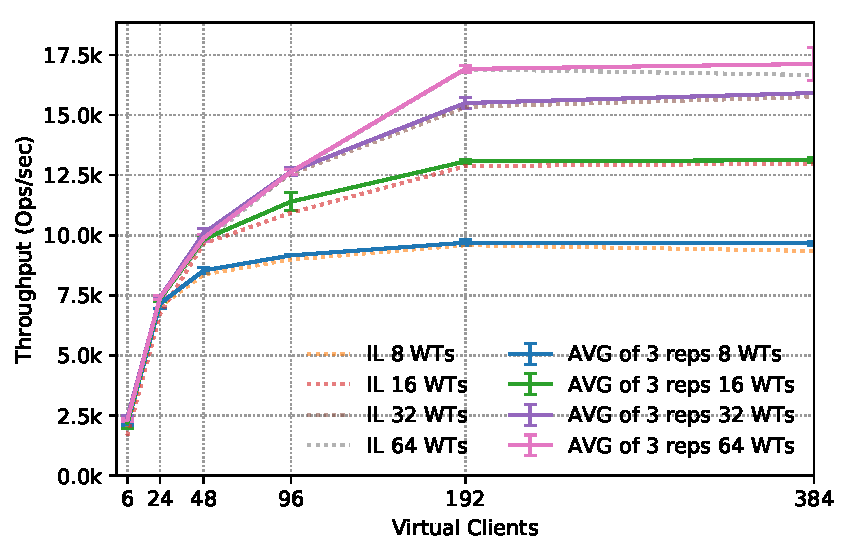
\includegraphics[width=0.6\textwidth]{figures/baseline_mw_2_mw/tp_memtier_write_only.pdf}
    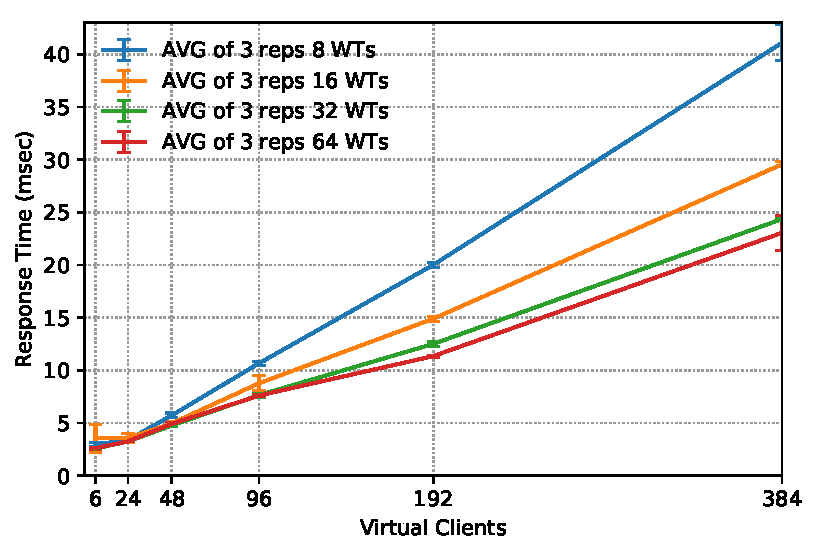
\includegraphics[width=0.6\textwidth]{figures/baseline_mw_2_mw/rt_memtier_write_only.pdf}
  }
\end{figure}

\begin{figure}[!h]
  \centering
  \caption{Plots for baseline with two Middlewares (write-only MIDDLEWARE)}
  \label{fig:baseline_mw_2_mw_mw_wo}
  \makebox[\textwidth]{
    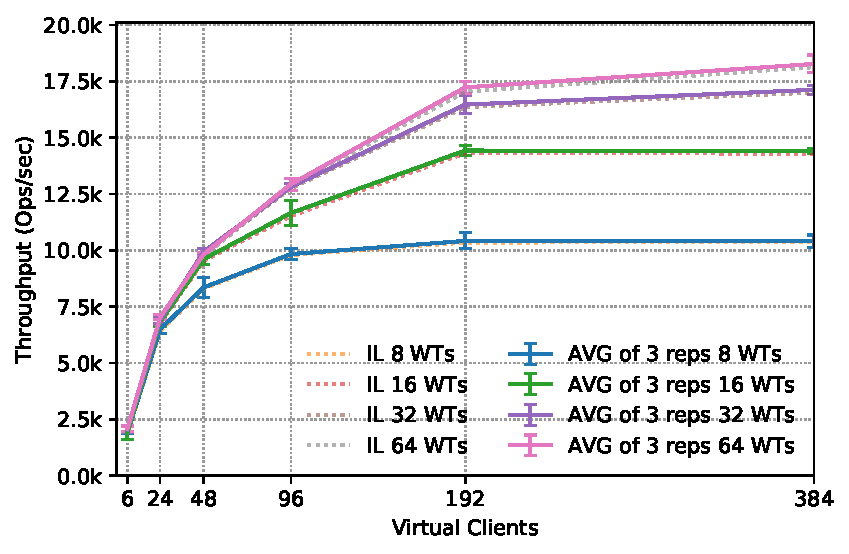
\includegraphics[width=0.6\textwidth]{figures/baseline_mw_2_mw/tp_middleware_write_only.pdf}
    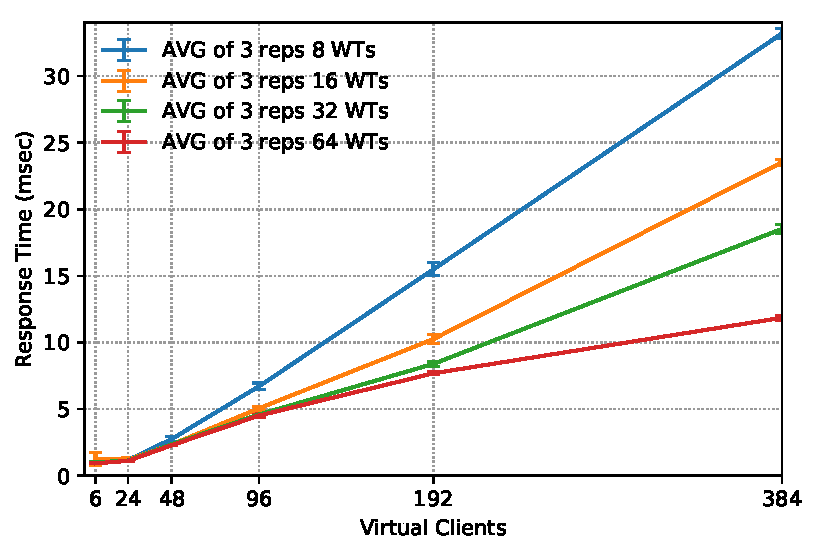
\includegraphics[width=0.6\textwidth]{figures/baseline_mw_2_mw/rt_middleware_write_only.pdf}
  }
\end{figure}

\begin{figure}[!h]
  \centering
  \caption{Plots for baseline with two Middlewares, Service Time and Queue Waiting Time (write-only MIDDLEWARE)}
  \label{fig:baseline_mw_2_mw_mw_c_wo}
  \makebox[\textwidth]{
    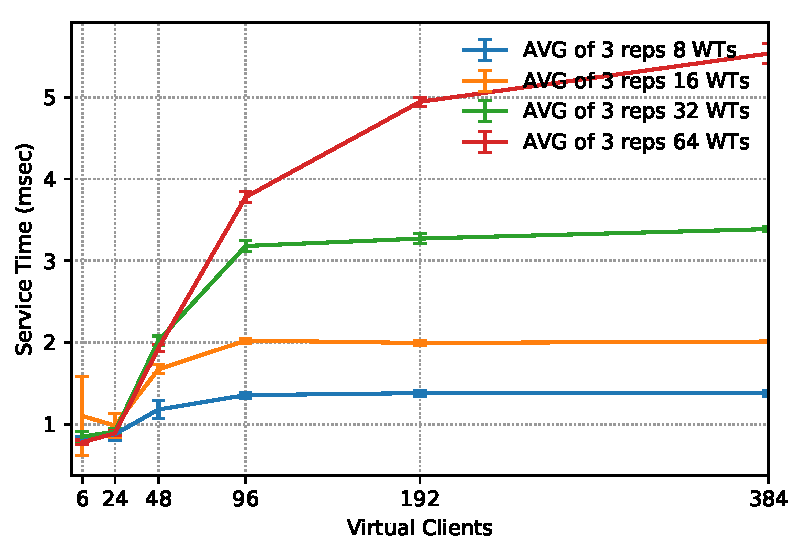
\includegraphics[width=0.6\textwidth]{figures/baseline_mw_2_mw/st_middleware_write_only.pdf}
    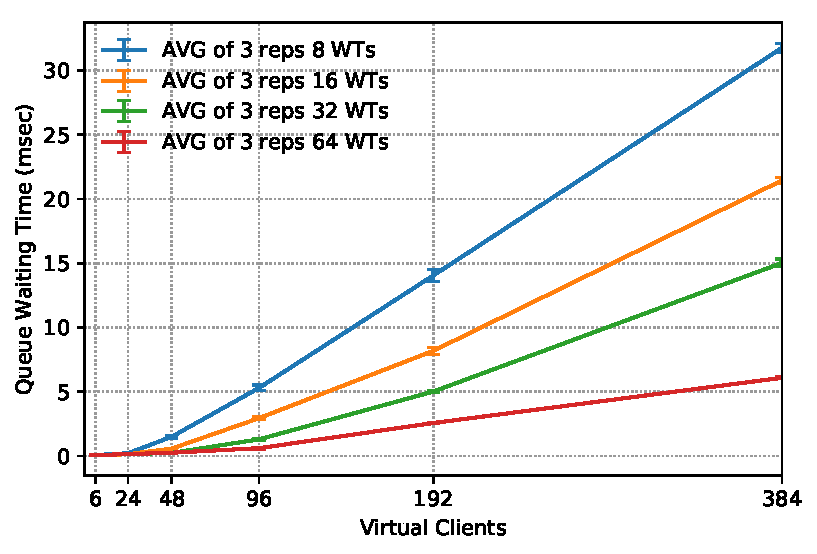
\includegraphics[width=0.6\textwidth]{figures/baseline_mw_2_mw/wt_middleware_write_only.pdf}
  }
\end{figure}

\begin{figure}[!h]
  \centering
    \caption{Plots for baseline with two Middlewares, Average Queue Size (write-only MIDDLEWARE)}
  \label{fig:baseline_mw_2_mw_mw_qs_wo}
  \makebox[\textwidth]{
    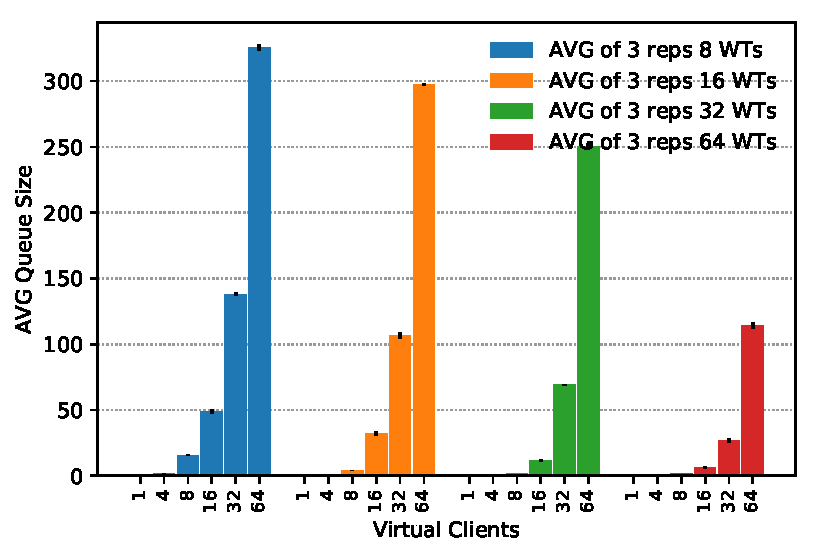
\includegraphics[width=0.6\textwidth]{figures/baseline_mw_2_mw/qs_middleware_write_only.pdf}
  }
\end{figure}

\subsection{Summary}

Based on the results obtained we can derive the following.

For the Baseline with one Middleware, for a read-only workload, the bottleneck is the memcached instance, which cannot output more than 3k $ops/s$, or $\approx 12 MB/s$.
For the write-only workload the bottleneck is the middleware, we can see a relevant drop in performance compared to Section \ref{sec:2.1}.

For the Baseline with two Middlewares, for a read-only workload, the bottleneck is still the memcached instance that cannot output more than 3k $ops/s$, indeed we doubled the number of middlwares compared to Section \ref{sec:3.1}, but the throughput doesn't seem to be affected at all, so it seems correct to blame the server for it.
In the write-only workload, we reach a similar performance as in Section \ref{sec:2.1}, the two middlewares don't affect performances, plus we know from Section \ref{sec:2.2} that a single client machine cannot send more than 6k $ops/s$ write-only requests, thus having 3 clients and reaching $\approx$ 18k $ops/s$ we can conclude that the bottleneck for this setup are the client machines.

\begin{center}
	{Maximum throughput for one middleware.}
	\begin{tabular}{|l|p{2cm}|p{2cm}|p{2cm}|p{2cm}|}
		\hline                                & Throughput & Response time & Average time in queue & Miss rate \\ 
		\hline Reads: Measured on middleware  & 2.92k $ops/s$ & 13.66 $ms$ & 0.85 $ms$ & 0.0 \\ 
        \hline Reads: Measured on clients     & 2.97k $ops/s$ & 16.22 $ms$ & n/a  & 0.0 \\ 
        \hline Writes: Measured on middleware & 12.5k $ops/s$ & 15.81 $ms$ & 10.42 $ms$ & n/a       \\ 
        \hline Writes: Measured on clients    & 12.7k $ops/s$ & 16.38 $ms$ & n/a & n/a       \\ 
		\hline 
	\end{tabular}
\end{center}

\begin{center}
	{Maximum throughput for two middlewares.}
	\begin{tabular}{|l|p{2cm}|p{2cm}|p{2cm}|p{2cm}|}
		\hline                                & Throughput & Response time & Average time in queue & Miss rate \\ 
		\hline Reads: Measured on middleware  & 2.95k $ops/s$ & 62.12 $ms$ & 22.15 $ms$            & 0.0       \\ 
		\hline Reads: Measured on clients     & 2.92k $ops/s$ & 64.32 $ms$ & n/a                   & 0.0       \\ 
		\hline Writes: Measured on middleware & 16.8k $ops/s$ & 8.25 $ms$ & 2.48 $ms$             & n/a       \\ 
        \hline Writes: Measured on clients    & 17.8k $ops/s$ & 11.43 $ms$ & n/a                   & n/a       \\ 
		\hline 
	\end{tabular}
\end{center}

\section{Throughput for Writes (90 pts)}
\label{sec:4.1}

\subsection{Full System}

\subsubsection*{Experiment Setting}

In this experiment we study the performance of the whole system when writing data.
The setup is the same as the one with two Middlewares in Section~\ref{sec:3.2}, we just increase the number of memcached machines to 3. Note that since we do not read data, we also do not need to populate the memcached servers.

\begin{center}
	\scriptsize{
		\begin{tabular}{|l|c|}
			\hline Number of servers                & 3          \\ 
			\hline Number of client machines        & 3          \\ 
			\hline Instances of memtier per machine & 2          \\ 
			\hline Threads per memtier instance     & 1          \\
			\hline Virtual clients per thread       & [1, 4, 8, 16, 24, 32, 64]    \\ 
			\hline Workload                         & Write-only \\
			\hline Multi-Get behavior               & N/A        \\
			\hline Multi-Get size                   & N/A        \\
			\hline Number of middlewares            & 2          \\
			\hline Worker threads per middleware    & [8, 16, 32, 64]    \\
            \hline Repetitions                      & 3 (70 secs, effective 60 secs) \\ 
            \hline Log Files Path                   & \texttt{experiments/throughput\_for\_writes/logs} \\
            \hline Processed Files Path             & \texttt{experiments/throughput\_for\_writes/out/memtier\_data.csv}\\
            \hline
		\end{tabular}
	} 
\end{center}

\subsubsection{Explanation}

The throughput plot is similar to the one in Section~\ref{sec:3.2}. Here we have thripled the number of servers, and throughput has noticeably decreased, at a point which it looks really similar to Section~\ref{sec:3.1}. This decrease is noticed also by looking at the measured response time. We can see how here, the maximum response time is $\approx$ 50 $ms$, (vs $\approx$ 40 $ms$ as in Figure \ref{fig:baseline_mw_2_mw_mw_wo}), and moreover, for every worker thread setup, the response time is shifted upwards, and at \texttt{VCs=384}, the difference between 8 and 64 worker threads is of $\approx$ 10 $ms$, smaller than the $\approx$ 15 $ms$ above.
This difference in response time is due to the fact that the service time in this setting has raised considerably: in the case of 8 workers we observe a growth of $\approx$ 1 $ms$, while with 64, more than $3ms$. 
Being the service time higher, each incoming request into the middleware spends more and more time waiting in the queue. This can be seen by comparing Figure \ref{fig:baseline_mw_1_mw_mw_c_wo} and Figure ~\ref{fig:throughput_for_writes_mw_c_wo}. We observe a constant increase of $\approx$ 10 $ms$ for every worker thread configuration. 
One can see how, for 8 and 16 worker threads the system is saturated already at \texttt{VCs=96}. With 32 worker threads the saturation point is reached with \texttt{VCs=144}, and with 64, at \texttt{VCs=192}.
Another evident behavior at those same point of saturation, is evident in the queue size plot: it starts to scale linearly as the workload increases, further confirming that the system is indeed saturated.

\subsubsection*{Write-Only}

\begin{figure}[!h]
  \centering
  \caption{Plots for throughput for writes (write-only CLIENT)}
    \label{fig:throughput_for_writes_mt_tp_wo}
  \makebox[\textwidth]{
    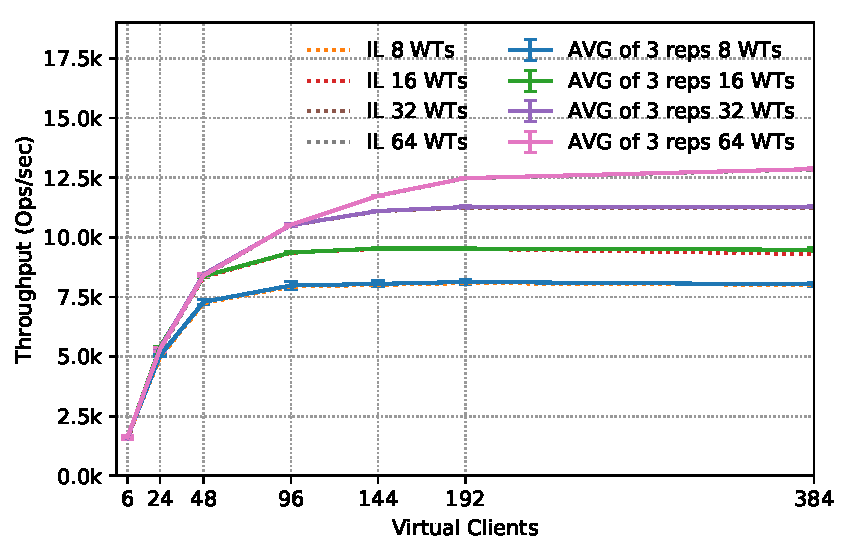
\includegraphics[width=0.6\textwidth]{figures/throughput_for_writes/tp_memtier_write_only.pdf}
    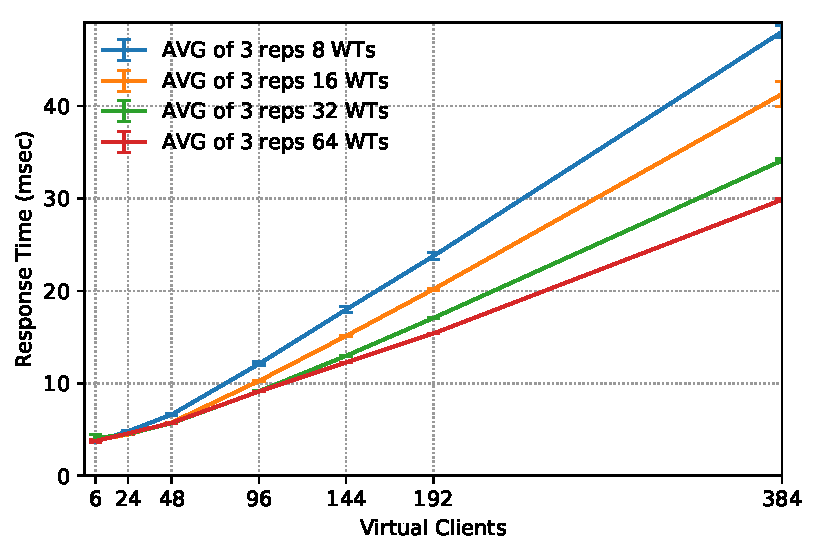
\includegraphics[width=0.6\textwidth]{figures/throughput_for_writes/rt_memtier_write_only.pdf}
  }
\end{figure}

\begin{figure}[!h]
  \centering
  \caption{Plots for throughput for writes (write-only MIDDLEWARE)}
    \label{fig:throughput_for_writes_mw_tp_wo}
  \makebox[\textwidth]{
    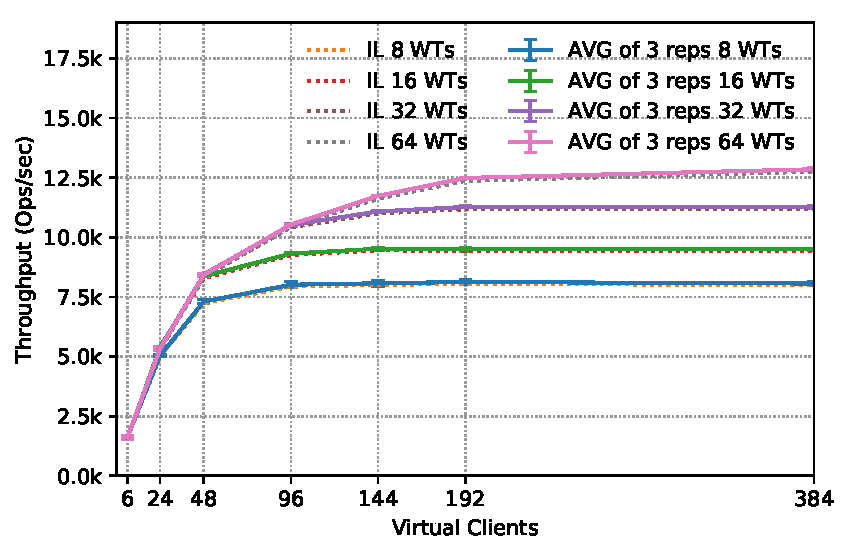
\includegraphics[width=0.6\textwidth]{figures/throughput_for_writes/tp_middleware_write_only.pdf}
    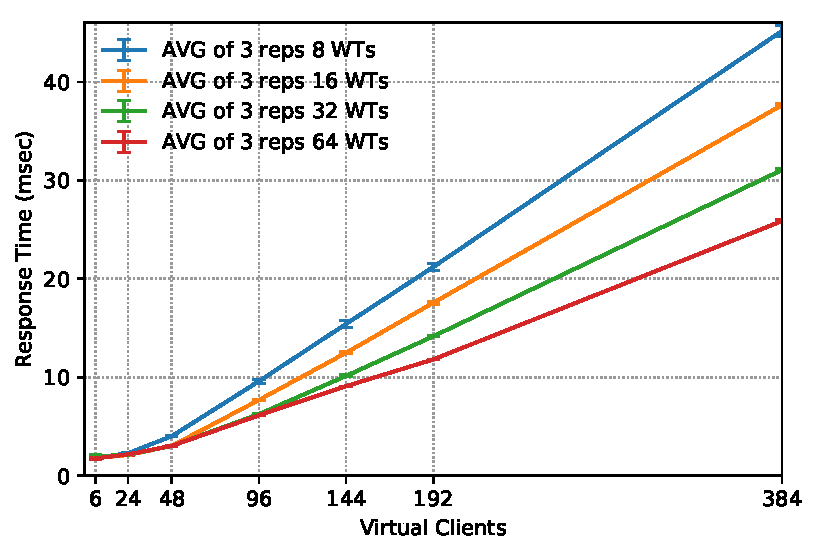
\includegraphics[width=0.6\textwidth]{figures/throughput_for_writes/rt_middleware_write_only.pdf}
  }
\end{figure}

\begin{figure}[!h]
  \centering
  \caption{Plots for throughput for writes, Service Time and Queue Waiting Time (write-only MIDDLEWARE)}
  \label{fig:throughput_for_writes_mw_c_wo}
  \makebox[\textwidth]{
    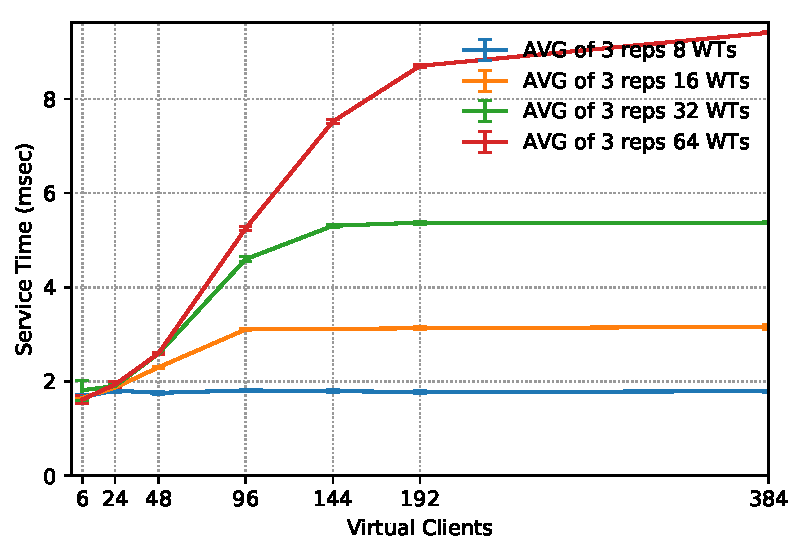
\includegraphics[width=0.6\textwidth]{figures/throughput_for_writes/st_middleware_write_only.pdf}
    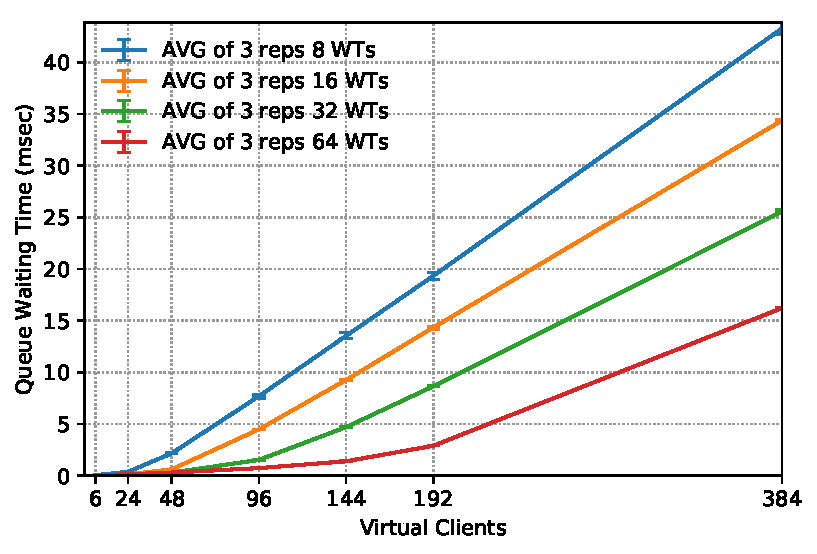
\includegraphics[width=0.6\textwidth]{figures/throughput_for_writes/wt_middleware_write_only.pdf}
  }
\end{figure}

\begin{figure}[!h]
  \centering
    \caption{Plots for throughput for writes, Average Queue Size (write-only MIDDLEWARE)}
    \label{fig:throughput_for_writes_mw_qs_wo}
  \makebox[\textwidth]{
    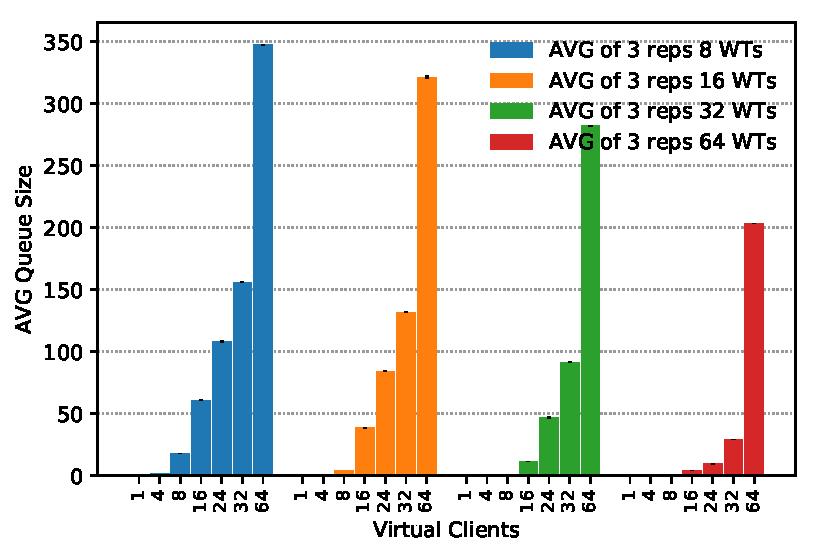
\includegraphics[width=0.6\textwidth]{figures/throughput_for_writes/qs_middleware_write_only.pdf}
  }
\end{figure}

\subsection{Summary}

Based on the results of this experiment we can derive the following.
In this configuration, when just performing write-only requests, the bottleneck are the two middlewares, more precisely, is the number of worker threads. 
The reason that supports this claim can be found by comparing Figure \ref{fig:throughput_for_writes_mw_tp_wo} and Figure \ref{fig:baseline_mw_2_mw_mw_wo}. In the latter, both middleware are connected to only one memcached instance, reaching a maximum trhoughput of $\approx$ 18k $ops/s$. Now, both middlewares are connected to 3 memcached instances, so if the middlewares would not represent a bottleneck we should reach a theoretical throughput 3 time bigger, but we don't, indeed we measure a substantial decrease. This can be explained by the fact  that there's some overhead when worker threads switch from a job to another, and also that when we perform writes, we need to wait for all 3 answers from the servers.\\


\begin{center}
	{Maximum throughput for the full system}
	\begin{tabular}{|l|p{1.5cm}|p{1.5cm}|p{1.5cm}|p{1.5cm}|}
		\hline                                            & WT=8         & WT=16        & WT=32         & WT=64         \\ 
		\hline Throughput (Middleware)                    & 8.3k $ops/s$ & 9.6k $ops/s$ & 11.3k $ops/s$ & 12.9k $ops/s$ \\ 
		\hline Throughput (Derived from MW response time) & 8.3k $ops/s$ & 9.6k $ops/s$ & 11.3k $ops/s$ & 12.9k $ops/s$ \\ 
		\hline Throughput (Client)                        & 8.3k $ops/s$ & 9.5k $ops/s$ & 11.3k $ops/s$ & 12.9k $ops/s$ \\ 
		\hline Average time in queue                      & 12.35 $ms$   & 9.04 $ms$    & 5.85 $ms$     & 3.11 $ms$     \\ 
		\hline Average length of queue                    & 49.4         & 41.4         & 30.9          & 17.6          \\ 
		\hline Average time waiting for memcached         & 1.77 $ms$    & 2.62 $ms$    & 3.85 $ms$     & 5.29 $ms$     \\ 
		\hline 
	\end{tabular}
\end{center}

\section{Gets and Multi-gets (90 pts)}

\subsection{Experiment Setting}

This set of experiments aims to measure and analyze the performance of the middleware when dealing with multi-GET requests.
There are 3 client machines running 2 single-threaded instances of memtier generating multi-GET workloads (as depicted in the table below). Each instance is connected two one of the two middlewares (each to a different one) with the maximum throughput configuration.
Each middleware is connected to 3 memcached machines running a single-threaded memcached instance each.
We are interested in generating two types of multi-GET requests (sharded and non-sharded), and compare their effect on the overall system.
We plot the throughput as measured in the middlewares, (not considering the number of $hits/s$), the average response time and its (25th, 50th, 75th, 90th and 99th) percentiles, and the distribution of response times (for the case of 6 keys) as measured by both memtier clients and the middlewares.

\subsection*{Maximum Throughput Choice}
For this particular case, since we are more concerned on the performances when reading rather than writing (which consitutes for a small fraction of the total of operations, $\approx \dfrac{1}{3 \cdot 6 \cdot 9}$), having no comparable setting (no experiment with 2 middlewares connected to 3 servers, apart from Section \ref{sec:4.1}), the maximum (stable) throughput considered is the one reached in \ref{sec:3.2}, obtained with 64 worker threads.

\subsection{Sharded Case}

\begin{center}
	\scriptsize{
		\begin{tabular}{|l|c|}
			\hline Number of servers                & 3                       \\ 
			\hline Number of client machines        & 3                       \\ 
			\hline Instances of memtier per machine & 2                       \\ 
			\hline Threads per memtier instance     & 1                       \\
			\hline Virtual clients per thread       & 2     		            \\ 
			\hline Workload                         & ratio=1:$<$Multi-Get size$>$             \\
			\hline Multi-Get behavior               & Sharded                 \\
			\hline Multi-Get size                   & [1, 3, 6, 9]            \\
			\hline Number of middlewares            & 2                       \\
            \hline Worker threads per middleware    & 64 (MAX throughput config) \\
            \hline Repetitions                      & 3 (70 secs, effective 60 secs) \\ 
            \hline Log Files Path                   & \texttt{experiments/multigets\_sharded/logs} \\
            \hline Processed Files Path             & \texttt{experiments/multigets\_sharded/out}\\
            \hline
		\end{tabular}
	} 
\end{center}

\subsubsection{Explanation}

By looking at the troughput plot, we can spot how the more keys we have in each request, the more the throughput decreases, starting from $\approx$ 3k $ops/s$ for the case of 1 key, to $\approx$ 2k $ops/s$ for the case with 9 keys. If we multiply the throughput by the number of keys, we obtain the number of $hits/s$ for each key configuration; that means approximately (3k, 8.4k, 14.4k, 17.5k) $hits/s$ for 1, 3, 6, and 9 keys respectively.
Thus we notice a gain in overall read performance by increasing the number of keys in a request.
When the number of keys is 3, for instance, compared to having 1 key, we almost thriple the number of $hits/s$ by thriplicating the number of servers we actually read from.\\
This gain though, doesn't seem to grow linearly if we compare the $hits/s$ with 3, 6 and 9 keys. With 6 keys, we are doubling the number of request for each of the 3 servers, and we obtain a slightly less number of $hits/s$ (8.4k $\cdot 2 = \approx 16.8$k $- 14.4$k $=2.2$k of difference). Same for 9 keys, (8.4 $\cdot 3 = \approx 25.2$k $-17.5$k $=7.7$k of difference).
The fact that the gain is not linear is better explained by looking at the reponse times for each key.
We can see how the average response time grows from $\approx 1.8 ms$ to $5.8 ms$ and how by increasing the number of keys, the percentiles also do. If we look at those for 1 and 3 keys, we observe how similar they are, meaning that the gap between the two average response times is explained by the latency of the 3 servers, instead of 1. Then if we compare 3 keys with 6, and 9 keys, we see a larger difference (especially for the 99th percentiles). This means that by increasing the load of each server, the service time also grow accordingly. In fact, if we break down the response time into the waiting time spent inside the queue, and into the time spent in service, we notice how effectively, the service time for 6 and 9 keys grows much more than in the case with 3 keys(Figure \ref{fig:multigets_sharded_mt_rt}).


\begin{figure}[!h]
  \centering
    \caption{Plots for multigets sharded, (Throughput MIDDLEWARE)}
  \label{fig:multigets_sharded_mw_tp}
  \makebox[\textwidth]{
    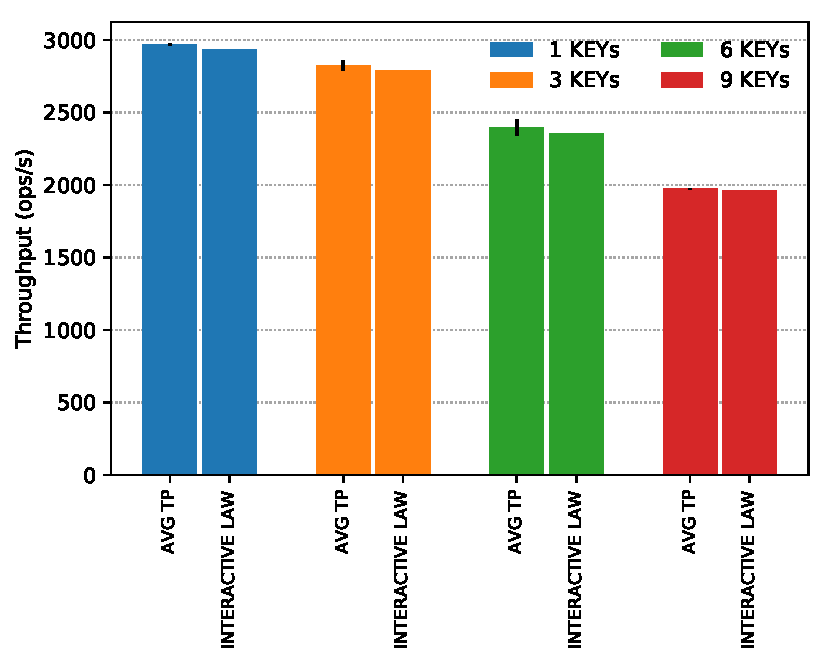
\includegraphics[width=0.6\textwidth]{figures/multigets_sharded/tp_middleware_multigets_sharded.pdf}
  }
\end{figure}

\begin{figure}[!h]
  \centering
    \caption{Plots for multigets sharded, (Response Time CLIENT, Response Time composition MIDDLEWARE)}
  \label{fig:multigets_sharded_mt_rt}
  \makebox[\textwidth]{
    \includegraphics[width=0.6\textwidth]{figures/multigets_sharded/rt_memtier_multigets_sharded.pdf}
    \includegraphics[width=0.6\textwidth]{figures/multigets_sharded/rt_breakdown_middleware_multigets_sharded.pdf}
  }
\end{figure}

\subsection{Non-sharded Case}

\subsection{Experiment Setting}

The only parameter that changes is the sharded flag, the rest of the configuration is the same as in the sharded case.

\begin{center}
	\scriptsize{
		\begin{tabular}{|l|c|}
			\hline Number of servers                & 3                       \\ 
			\hline Number of client machines        & 3                       \\ 
			\hline Instances of memtier per machine & 2                       \\ 
			\hline Threads per memtier instance     & 1                       \\
			\hline Virtual clients per thread       & 2                		 \\ 
			\hline Workload                         & ratio=1:$<$Multi-Get size$>$              \\
			\hline Multi-Get behavior               & Non-Sharded             \\
			\hline Multi-Get size                   & [1, 3, 6, 9]                  \\
			\hline Number of middlewares            & 2                       \\
            \hline Worker threads per middleware    & 64 (MAX throughput config) \\
            \hline Repetitions                      & 3 (70 secs, effective 60 secs) \\ 
            \hline Log Files Path                   & \texttt{experiments/multigets\_non\_sharded/logs} \\
            \hline Processed Files Path             & \texttt{experiments/multigets\_non\_sharded/out/memtier\_data.csv}\\
            \hline
		\end{tabular}
	} 
\end{center}

\subsubsection{Explanation}

We analyze the throughput plot as we have done for the sharded case. So if we consider the number of $hits/s$ again we approximately have: (2.75k, 7.5k, 6k, 16.2k) $hits/s$ for (1, 3, 6 and 9) keys respectively.
For 1 key, the standard deviation seems higher than before, but we still get a close measure. 
That can be said also for the other keys, although by growing the number of keys, the difference compared to the sharded case seems to be in the range of 1k to 2k $hits/s$
Interestingly, how the average response time doesn't grow much the same as in the sharded case. We notice a growth of the 75th, 90th, and 99th percentiles by $\approx$ 2-3 $ms$.
This growth is noticeable if we look into the response time composition plot: here we can see how both service time and waiting time have slighlty raised compared to the sharded case.

\begin{figure}[!h]
  \centering
    \caption{Plots for multigets non sharded, (Throughput MIDDLEWARE)}
  \label{fig:multigets_non_sharded_mw_tp}
  \makebox[\textwidth]{
      \includegraphics[width=0.6\textwidth]{figures/multigets_non_sharded/tp_middleware_multigets_non_sharded.pdf}
  }
\end{figure}

\begin{figure}[!h]
  \centering
    \caption{Plots for multigets non sharded, (Response Time CLIENT, Response Time composition MIDDLEWARE)}
  \label{fig:multigets_non_sharded_mt_rt}
  \makebox[\textwidth]{
    \includegraphics[width=0.6\textwidth]{figures/multigets_non_sharded/rt_memtier_multigets_non_sharded.pdf}
    \includegraphics[width=0.6\textwidth]{figures/multigets_non_sharded/rt_breakdown_middleware_multigets_non_sharded.pdf}
  }
\end{figure}

\subsection{Histogram}

\begin{figure}[!h]
  \centering
    \caption{Plots for multigets sharded, (Response Time Distribution CLIENT \& MIDDLEWARE)}
  \label{fig:multigets_sharded_mt_mw_rt_d}
  \makebox[\textwidth]{
    \includegraphics[width=0.6\textwidth]{figures/multigets_sharded/rt_distribution_memtier_multigets_sharded.pdf}
    \includegraphics[width=0.6\textwidth]{figures/multigets_sharded/rt_distribution_middleware_multigets_sharded.pdf}
  }
\end{figure}

\begin{figure}[!h]
  \centering
    \caption{Plots for multigets non sharded, (Response Time Distribution CLIENT \& MIDDLEWARE)}
  \label{fig:multigets_non_sharded_mt_mw_rt_d}
  \makebox[\textwidth]{
    \includegraphics[width=0.6\textwidth]{figures/multigets_non_sharded/rt_distribution_memtier_multigets_non_sharded.pdf}
    \includegraphics[width=0.6\textwidth]{figures/multigets_non_sharded/rt_distribution_middleware_multigets_non_sharded.pdf}
  }
\end{figure}

We plot the distribution of the response times measured for the 6-key configuration at the clients and inside the middlwares.
For both the client and the middleware, the distribution is obtained as the aggregate distribution of all runs with 6 keys. We show just the first $30 ms$ interval for visual purposes, (as it would be too spreaded and flatconsidering the whole distribution). The number of bins is 30, so each bin covers a $1 ms$ interval.
Visually there seems to be not too much difference if we compare the sharded and non sharded scenarios, although the non-sharded one present higher bars in the 10-15 interval range.
If we compare the client plots with the middleware, we can see the difference in the measured response time (depicted in Section~\ref{sec:3.1}, as the shift in the bars.

\subsection{Summary}

Based on what presented above we derive the following. \\
Sharding, seems to be the preferable option with 1, 3, 6 and 9 keys (no relevant difference with 1 key).
From plotting the composition of the response times, we have seen that majority of the time a multi-GET request spends inside the system is given by the service time of the servers.
From that, it seems that the sharding operation inside the middleware is almost irrelevant in the composition of the response time, (beacuse service time timing starts when the request leaves the middleware).

\section{2K Analysis (90 pts)}

We perform a $2^kr$ experimental analysis to investigate the effect of ($k=3$) \textbf{factors}, namely:

\begin{itemize}
    \item The number of memcached servers
    \item The number of middlewares
    \item The number of worker threads per middleware
\end{itemize}

and study the effects of each of them on throughput and response time respectively (\textbf{response variables}).

\subsection{Experiment setting}

There are 3 machines that generate write-only and read-only workloads. Then based on the number of middlewares (1 or 2), each client machine runs (1 or 2) instances of memtier, each with 32 virtual clients and (2 or 1) threads respectively. In the case of two memtier instances per machine, each of them connects to a different middleware. 
Each middleware runs either (8 or 32) worker threads, and is connected to either (2 or 3) mecached machines. We measure both throughput and response time for each workload (read-only and write-only).
We investigate experimental errors by replicating each experiment 3 times ($r=3$), so the response variable, is simply the average between each repetition.
Based on results on experiments in Section~\ref{sec:3.1}, we do expect the number of middlewares and the number of worker threads, to have relevant impact on the response variables. Furthermore, we do assume that the effects of the factor are additive and that measurements error are independent and follow a normal distribution.\\

\begin{center}
	\scriptsize{
		\begin{tabular}{|l|c|}
			\hline Number of servers                & 1 and 3                                     \\ 
			\hline Number of client machines        & 3                                           \\ 
			\hline Instances of memtier per machine & 1 (1 middleware) or 2 (2 middlewares) \\ 
			\hline Threads per memtier instance     & 2 (1 middleware) or 1 (2 middlewares)   \\
			\hline Virtual clients per thread       &  32                                     \\ 
			\hline Workload                         & Write-only and Read-only\\
			\hline Multi-Get behavior               & N/A                                         \\
			\hline Multi-Get size                   & N/A                                         \\
			\hline Number of middlewares            & 1 and 2                                     \\
			\hline Worker threads per middleware    & 8 and 32                                    \\
			\hline Repetitions                      & 3 or more (at least 1 minute each)                                   \\ 
			\hline 
		\end{tabular}
	} 
\end{center}

\subsection{Model}

We model the response variable $y$ as\\
\begin{equation}
    y = q_0 + q_Ax_A + q_Bx_B + q_Cx_C + q_{AB}x_Aa_B + q_{AC}x_Ax_C + q_{BC}x_Bx_C + q_{ABC}x_Ax_Bx_C + \epsilon
\end{equation}

where $x_A, x_B, x_C$ are defined as\\
\begin{align*}
x_A &= 
\begin{cases}
    -1 & \text{ if 1 server}\\
    1 & \text{ if 3 servers}
\end{cases}
\\
x_B &=
\begin{cases}
    -1 & \text{ if 1 middleware}\\
    1 & \text{ if 2 middlewares}
\end{cases}
\\
x_C &=
\begin{cases}
    -1 & \text{ if 8 worker threads}\\
    1 & \text{ if 32 worker threads}
\end{cases}
\end{align*}

and $q_0, q_A, \dots q_{ABC},$ and $\epsilon$ (\textbf{experimental error}) are the parameters to be computed with the \textit{Sign Table Method}.

\subsection{Results}

\subsubsection*{Throughput}

\subsubsection*{Read-Only}

\begin{table}[!htb]
    \centering
    \caption{Sign Table Method for read-only workload (Throughput)}
\scriptsize{
\begin{tabu}{|r|r|r|r|r|r|r|r|r|r|r|r|r|}
\hline
    \rowfont[c]{\bfseries} i & I & A & B & C & AB & AC & BC & ABC & $y_1$ & $y_2$ & $y_3$ & $\hat{y}$\\ \hline
    1 & 1 & -1 & -1 & -1 & 1 & 1 & 1 & -1 & 2919.15 & 2924.77 & 2926.62 & 2923.51\\ \hline
    2 & 1 & -1 & -1 & 1 & 1 & -1 & -1 & 1 & 2938.38 & 2941.38 & 293985 & 2939.87\\ \hline
    3 & 1 & -1 & 1 & -1 & -1 & 1 & -1 & 1 & 2931.00 & 2930.24 & 2936.23 & 2932.49\\ \hline
    4 & 1 & -1 & 1 & 1 & -1 & -1 & 1 & -1 & 2930.93 & 2935.77 & 2943.00 & 2936.57\\ \hline
    5 & 1 & 1 & -1 & -1 & -1 & -1 & 1 & 1 & 2208.15 & 2100.92 & 2105.38& 2138.15\\ \hline
    6 & 1 & 1 & -1 & 1 & -1 & 1 & -1 & -1 & 2329.69 & 2279.54 & 2379.46 & 2329.56\\ \hline
    7 & 1 & 1 & 1 & -1 & 1 & -1 & -1 & -1 & 4051.39 & 4144.38 & 3912.92 & 4036.23\\ \hline
    8 & 1 & 1 & 1 & 1 & 1 & 1 & 1 & 1 & 4391.15 & 4464.54 & 4362.77 & 4406.15\\ \hline
      & 3080.32 & 147.21 & 497.54 & 72.72 & 496.12 & 67.61 & 20.78 & 23.85 & Total/8 & & &\\ \hline
\end{tabu}
}
\end{table}

In the above table, each row represents one combination of the factors ($x_A, x_B, x_C$), the last column
is the average throughput and, the last row in the table shows the coefficients ($q_0, q_A, \dots q_ABC$) that solve the system of equations.

\begin{table}[!htb]
  \centering
    \caption{Allocation of variations for read-only workload (Throughput)}
  \label{tab:ro_variation}
  \small{
    \begin{tabular}{|l|r|r|}
        \hline \textbf{Sum}   & \textbf{Value}        & \textbf{\% / SST} \\
      \hline SS0   & 227720480.01 & N/A      \\
      \hline SSA   & 520078.21    & 4.10\%  \\
      \hline SSB   & 5941174.89   & 46.88\% \\
      \hline SSC   & 126921.12    & 1.00\% \\
      \hline SSAB  & 5907350.45   & 46.61\%  \\
      \hline SSAC  & 109716.16    & 0.87\%  \\
      \hline SSBC  & 10362.15     & 0.08\%  \\
      \hline SSABC & 13650.31     & 0.11\%  \\
      \hline SSE   & 45129.63     & 0.356\%  \\
      \hline SST   & 12674382.93  & 100.00\% \\
      \hline SSY   & 240394862.94 & N/A      \\
      \hline
    \end{tabular}
  }
\end{table}


\newpage
\subsubsection*{Write-Only}

\begin{table}[!htb]
    \centering
    \caption{Sign Table Method for write-only workload (Throughput)}
\scriptsize{
\begin{tabu}{|r|r|r|r|r|r|r|r|r|r|r|r|r|}
\hline
    \rowfont[c]{\bfseries} i & I & A & B & C & AB & AC & BC & ABC & $y_1$ & $y_2$ & $y_3$ & $\hat{y}$\\ \hline
    1 & 1 & -1 & -1 & -1 & 1 & 1 & 1 & -1 & 7513.69 & 7467.46 & 7527.77 & 7502.97\\ \hline
    2 & 1 & -1 & -1 & 1 & 1 & -1 & -1 & 1 & 10299.85 & 10494.08 & 10384.38 & 10392.77\\ \hline
    3 & 1 & -1 & 1 & -1 & -1 & 1 & -1 & 1 & 10539.31 & 11077.77 & 11350.31 & 10989.13\\ \hline
    4 & 1 & -1 & 1 & 1 & -1 & -1 & 1 & -1 & 15661.00 & 15949.92 & 15640.54 & 15753.82\\ \hline
    5 & 1 & 1 & -1 & -1 & -1 & -1 & 1 & 1 & 4942.85 & 4501.46 & 5197.00 & 4880.44\\ \hline
    6 & 1 & 1 & -1 & 1 & -1 & 1 & -1 & -1 & 7163.38 & 6809.62 & 6746.46 & 6912.49\\ \hline
    7 & 1 & 1 & 1 & -1 & 1 & -1 & -1 & -1 & 6719.23 & 7008.00 & 7159.15 & 6962.13\\ \hline
    8 & 1 & 1 & 1 & 1 & 1 & 1 & 1 & 1 & 10302.61 & 10609.69 & 10622.93 & 10511.74\\ \hline
      & 9238.19 & -1921.49 & 1816.02 & 1654.52 & -395.78 & -259.1 & 424.06 & -44.67 & Total/8 & & &\\ \hline
\end{tabu}
}
\end{table}

\begin{table}[!htb]
  \centering
    \caption{Allocation of variations for write-only workload (Throughput)}
  \label{tab:wo_variation}
  \small{
    \begin{tabular}{|l|r|r|}
        \hline \textbf{Sum}   & \textbf{Value}        & \textbf{\% / SST} \\
      \hline SS0   & 2048257859.79 & N/A      \\
      \hline SSA   & 88610741.10   & 36.298\%  \\
      \hline SSB   & 79150214.73   & 32.4\% \\
      \hline SSC   & 65698408.15   & 26.91\% \\
      \hline SSAB  & 3759450.90    & 1.54\%  \\
      \hline SSAC  & 1611218.53    & 0.66\%  \\
      \hline SSBC  & 4315794.32    & 1.768\%  \\
      \hline SSABC & 47880.88      & 0.02\%  \\
      \hline SSE   & 928128.86     & 0.38\%  \\
      \hline SST   & 244121837.47  & 100.00\% \\
      \hline SSY   & 2292379697.26 & N/A      \\
      \hline
    \end{tabular}
  }
\end{table}

\subsubsection*{ResponseTime}

\subsubsection*{Read-Only}

\begin{table}[!htb]
    \centering
    \caption{Sign Table Method for read-only workload (Response Time)}
\begin{tabu}{|r|r|r|r|r|r|r|r|r|r|r|r|r|}
\hline
    \rowfont[c]{\bfseries} i & I & A & B & C & AB & AC & BC & ABC & $y_1$ & $y_2$ & $y_3$ & $\hat{y}$\\ \hline
    1 & 1 & -1 & -1 & -1 & 1 & 1 & 1 & -1 & 62.73 & 62.47 & 62.54 & 62.58\\ \hline
    2 & 1 & -1 & -1 & 1 & 1 & -1 & -1 & 1 & 62.01 & 61.87 & 61.47 & 61.68\\ \hline
    3 & 1 & -1 & 1 & -1 & -1 & 1 & -1 & 1 & 63.30 & 63.26 & 63.14 & 63.23\\ \hline
    4 & 1 & -1 & 1 & 1 & -1 & -1 & 1 & -1 & 62.57 & 62.45 & 62.33 & 62.45\\ \hline
    5 & 1 & 1 & -1 & -1 & -1 & -1 & 1 & 1 & 78.62 & 85.91 & 83.73 & 82.75\\ \hline
    6 & 1 & 1 & -1 & 1 & -1 & 1 & -1 & -1 & 60.64 & 63.64 & 61.04 & 61.77\\ \hline
    7 & 1 & 1 & 1 & -1 & 1 & -1 & -1 & -1 & 42.02 & 41.22 & 44.16 & 42.46\\ \hline
    8 & 1 & 1 & 1 & 1 & 1 & 1 & 1 & 1 & 32.84 & 32.94 & 33.53 & 33.10\\ \hline
      & 58.77 & -3.74 & -8.46 & -3.99 & -8.78 & -3.60 & 1.45 & 1.45 & Total/8 & & &\\ \hline 
\end{tabu}
\end{table}

\begin{table}[!htb]
  \centering
    \caption{Allocation of variations for read-only workload (Response Time)}
  \label{tab:wo_variation}
  \small{
    \begin{tabular}{|l|r|r|}
        \hline \textbf{Sum}        & \textbf{Value}        & \textbf{\% / SST} \\
      \hline SS0   & 82882.74      & N/A      \\
      \hline SSA   & 336.41        & 7.102\%  \\
      \hline SSB   & 1716.28       & 32.4\% \\
      \hline SSC   & 382.12        & 8.067\% \\
      \hline SSAB  & 1852.14       & 39.101\%  \\
      \hline SSAC  & 310.21        & 6.549\%  \\
      \hline SSBC  & 50.74         & 1.071\%  \\
      \hline SSABC & 50.50         & 1.066\%  \\
      \hline SSE   & 38.44         & 0.812\%  \\
      \hline SST   & 4736.85       & 100.00\% \\
      \hline SSY   & 87619.6       & N/A      \\
      \hline
    \end{tabular}
  }
\end{table}

\newpage
\subsubsection*{Write-Only}

\begin{table}[!htb]
    \centering
    \caption{Sign Table Method for write-only workload (Response Time)}
\begin{tabu}{|r|r|r|r|r|r|r|r|r|r|r|r|r|}
\hline
    \rowfont[c]{\bfseries} i & I & A & B & C & AB & AC & BC & ABC & $y_1$ & $y_2$ & $y_3$ & $\hat{y}$\\ \hline
    1 & 1 & -1 & -1 & -1 & 1 & 1 & 1 & -1 & 20.16 & 22.01 & 20.56 & 20.91\\ \hline
    2 & 1 & -1 & -1 & 1 & 1 & -1 & -1 & 1 & 11.71 & 9.43 & 11.99 & 11.04\\ \hline
    3 & 1 & -1 & 1 & -1 & -1 & 1 & -1 & 1 & 15.60 & 14.74 & 14.06 & 14.80\\ \hline
    4 & 1 & -1 & 1 & 1 & -1 & -1 & 1 & -1 & 9.00 & 8.75 & 8.85 & 8.87\\ \hline
    5 & 1 & 1 & -1 & -1 & -1 & -1 & 1 & 1 & 35.89 & 34.65 & 34.07 & 34.87\\ \hline
    6 & 1 & 1 & -1 & 1 & -1 & 1 & -1 & -1 & 22.1 & 23.53 & 21.51 & 22.38\\ \hline
    7 & 1 & 1 & 1 & -1 & 1 & -1 & -1 & -1 & 25.4 & 24.73 & 24.24 & 24.79\\ \hline
    8 & 1 & 1 & 1 & 1 & 1 & 1 & 1 & 1 & 15.76 & 15.10 & 15.03 & 15.30\\ \hline
      & 19.12 & 5.21 & -3.18 & -4.72 & -1.11 & 0.77 & 0.87 & -0.12 & Total/8 & & &\\ \hline
\end{tabu}
\end{table}

\begin{table}[!htb]
  \centering
    \caption{Allocation of variations for write-only workload (Response Time)}
  \label{tab:wo_variation}
  \small{
    \begin{tabular}{|l|r|r|}
        \hline \textbf{Sum}   & \textbf{Value}        & \textbf{\% / SST} \\
      \hline SS0   & 8772.45       & N/A      \\
      \hline SSA   & 652.66        & 43.361\%  \\
      \hline SSB   & 243.05        & 16.147\% \\
      \hline SSC   & 535.30        & 35.563\% \\
      \hline SSAB  & 29.54         & 1.962\%  \\
      \hline SSAC  & 14.35         & 0.953\%  \\
      \hline SSBC  & 18.02         & 1.197\%  \\
      \hline SSABC & 0.33          & 0.022\%  \\
      \hline SSE   & 11.95         & 0.794\%  \\
      \hline SST   & 1505.18       & 100.00\% \\
      \hline SSY   & 10277.63      & N/A      \\
      \hline
    \end{tabular}
  }
\end{table}

\newpage
\section{Queuing Model (90 pts)}

In this section we model our system with different techniques using some particular measurements recorded inside the middleware, to predict the behavior of the internal state of the system, and compare it, with the actual values.

In this section we introduce the following notation to describe the relevant factors that we take into consideration:

\begin{itemize}
    \item $\tau$ is the interarrival time between two successive requests
    \item $\lambda$ is the arrival rate
    \item $\mu$ is the service rate
    \item $\rho$ is the utilization factor
    \item $\varrho$ is the probability of queueing
    \item $r$ is the response time
    \item $s$ is the service time
    \item $w$ is the queue waiting time
    \item $n$ is the total number of jobs in the system ($n = n_q + n_s$)
    \item $n_q$ is the total number of jobs waiting in the queue
    \item $n_s$ is the total number of jobs being served
\end{itemize}

\subsection{M/M/1}

In this section we model our system based on the results of Section~\ref{sec:4.1} for each worker thread configuration.
In the M/M/1 model ther is only a single queue and a single server ($m=1$). The model assumes that the $\tau$'s are IID, (follow a Poisson distribution: meaning constant rate and independence between each sample), and that jobs get enqueued in a single queue from where they get taken out and serviced in a First Come, Fist Served fashion. Another assumption of the model is that, it is closed, meaning that no flow can enter from outside; thus we can already take the throughput as a measure of $\lambda$, (indeed memtier machines issue new request upon receiving an answer back for the current request being serviced). 
In order to conduct further analysis we need to estimate the service rate $\mu$. We could either:
\begin{itemize}
    \item compute the service rate as the inverse of the mean service time. If we would choose this approach, we would need to into account that we are running two middlewares with 64 worker threads so we should normalize the service time by dividing it for $(\#mws \cdot \#wts$) so 128 in this case.
    \item use the maximum measured throughput as lower bound on the service rate. This is justified by the fact that the average throughput is always less or equal the average service rate in our system, given the fact that wait some idle in the queue. Moreover there's some overhead created by switching jobs, so it seems a fair reasonable measure.
\end{itemize}
We try both approaches and compared the results in the following Section.
As $\lambda$ depends on the number of virtual clients, we choose to report the results we obtain for two configurations: one with \texttt{VCs=24} (under-saturated system), and one with \texttt{VCs=384} (saturated system). 

\begin{table}[!h]
  \centering
    \caption{Results of the M/M/1 queue model for 24 \texttt{VCs}. Service rate is tha max throughput measured. Gray values represent actual measurements.}
  \label{tab:mm124}
  \makebox[\textwidth]{
    \small{
      \begin{tabular}{|l|r|r|r|r|}
        \hline                                                    & WT = 8           & WT = 16          & WT = 32          & WT = 64          \\
        \hline Arrival rate ($\lambda$)                           & 5.04k $ops/s$    & 5.4k $ops/s$     & 5.3k $ops/s$     & 5.3k $ops/s$     \\
        \hline Average time waiting for memcached                 & 2.29 $ms$        & 2.11 $ms$        & 2.14 $ms$        & 2.117 $ms$       \\
        \hline Service Rate ($\mu$, from adjusted service time)   & 5073 ${reqs/s}$      & 5439 ${reqs/s}$      & 5377 ${reqs/s}$      & 5390 ${reqs/s}$      \\
        \hline Utilization ($\rho$)                               & 0.99             & 0.99             & 0.98             & 0.98             \\
        \hline Mean \# of jobs in the system ($E[n]$)             & 199.8 ${reqs}$       & 143.04 ${reqs}$      & 237.67 ${reqs}$      & 92.14 ${reqs}$       \\
        \hline Mean \# of jobs in the queue ($E[n_q]$)            & 198.8${reqs}$        & 141.04 ${reqs}$      & 236.67 ${reqs}$      & 91.15 ${reqs}$       \\
        \hline Mean response time ($E[r]$)                        & 39.5 ${ms}$          & 26.4 ${ms}$          & 44.35 ${ms}$         & 17.2 ${ms}$          \\
        \hline Mean waiting time ($E[w]$)                         & 39.3 ${ms}$          & 26.3 ${ms}$          & 44.19 ${ms}$         & 17.09 ${ms}$         \\
        \rowcolor{mygray}
        \hline Mean \# of jobs in the system ($E[n]$)             & $\approx$ 0.11 ${reqs}$ & $\approx$ 0.15 ${reqs}$ & $\approx$ 0.28 ${reqs}$ & $\approx$ 0.43 ${reqs}$ \\
        \rowcolor{mygray}
        \hline Mean \# of jobs in the queue ($E[n_q]$)            & 1.3 ${reqs}$         & 2.7 ${reqs}$         & 5.8 ${reqs}$         & 13.8 ${reqs}$        \\
        \rowcolor{mygray}
        \hline Mean response time ($E[r]$)                        & 1.53 ${ms}$          & 1.98 ${ms}$          & 3.75 ${ms}$          & 5.8 ${ms}$           \\
        \rowcolor{mygray}
        \hline Mean waiting time ($E[w]$)                         & 0.16 ${ms}$          & 0.27 ${ms}$          & 0.81 ${ms}$          & 1.44 ${ms}$          \\
        \hline
      \end{tabular}
    }
  }
\end{table}


\begin{table}[!h]
  \centering
    \caption{Results of the M/M/1 queue model for 384\texttt{VCs}. Service rate is tha max throughput measured. Gray values represent actual measurements.}
  \label{tab:mm1384}
  \makebox[\textwidth]{
    \small{
      \begin{tabular}{|l|r|r|r|r|}
        \hline                                                    & WT = 8           & WT = 16          & WT = 32          & WT = 64           \\
        \hline Arrival rate ($\lambda$)                           & 8.06k $ops/s$    & 9.5k $ops/s$     & 11.2k $ops/s$    & 12.8k $ops/s$     \\
        \hline Average time waiting for memcached                 & 1.79 $ms$        & 3.16 $ms$        & 5.37 $ms$        & 9.4 $ms$          \\
        \hline Service Rate ($\mu$, from adjusted service time)   & 8.18k ${reqs/s}$     & 9.5k ${reqs/s}$      & 11.36k reqs/     & 12.9k ${reqs/s}$      \\
        \hline Utilization ($\rho$)                               & 0.98             & 0.99             & 0.98             & 0.98              \\
        \hline Mean \# of jobs in the system ($E[n]$)             & 83.96 ${reqs}$       & 278.5 ${reqs}$       & 282.2 ${reqs}$      & 203.4 ${reqs}$        \\
        \hline Mean \# of jobs in the queue ($E[n_q]$)            & 82.9 ${reqs}$        & 277.5 ${reqs}$       & 139.02 ${reqs}$      & 167.4 ${reqs}$        \\
        \hline Mean response time ($E[r]$)                        & 10.41 ${ms}$         & 29.3 ${ms}$          & 12.4 ${ms}$          & 13.11 ${ms}$          \\
        \hline Mean waiting time ($E[w]$)                         & 10.29 ${ms}$         & 29.2 ${ms}$          & 12.32 ${ms}$         & 13.03 ${ms}$          \\
        \rowcolor{mygray}
        \hline Mean \# of jobs in the system ($E[n]$)             & 5.2 ${reqs}$       & 5.1 ${reqs}$       & 14.96 ${reqs}$      & 4.73 ${reqs}$        \\
        \rowcolor{mygray}
        \hline Mean \# of jobs in the queue ($E[n_q]$)            & 347.36 $reqs$      & 321.46 $reqs$      & 282.2 $reqs$       & 203.4 $reqs$        \\
        \rowcolor{mygray}
        \hline Mean response time ($E[r]$)                        & 45.17 $ms$         & 37.6 $ms$          & 31.05 $ms$         & 25.87 $ms$          \\
        \rowcolor{mygray}
        \hline Mean waiting time ($E[w]$)                         & 43.29 $ms$         & 34.3 $ms$          & 25.56 $ms$         & 16.23 $ms$          \\
        \hline
      \end{tabular}
    }
  }
\end{table}

\subsection{M/M/m}

\begin{table}[!h]
  \centering
    \caption{Results of the M/M/m queue model for 24 \texttt{VCs}}
  \label{tab:mmm24}
  \makebox[\textwidth]{
    \small{
      \begin{tabular}{|l|r|r|r|r|}
        \hline                                                    & WT = 8        & WT = 16             & WT = 32              & WT = 64          \\
        \hline Arrival rate ($\lambda$)                           & 5.04k $ops/s$ & 5.4k $ops/s$        & 5.3k $ops/s$         & 5.3k $ops/s$     \\
        \hline Average time waiting for memcached                 & 2.29 $ms$     & 2.11 $ms$           & 2.14 $ms$            & 2.117 $ms$       \\
          \hline Service Rate ($\mu$)                             & 552 ${reqs/s}$& 534 ${reqs/s}$      & 524 ${reqs/s}$       & 516 ${reqs/s}$      \\
        \hline Utilization ($\rho$)                               & 0.57          & 0.31                & 0.15                 & 0.08             \\
          \hline Probability of queuing ($\varrho$)               & 0.03          & 3.14 $e-8$          & 1.24 $e-29$          & 5.17 $e-91$           \\
        \hline Mean \# of jobs in the system ($E[n]$)             & 9.17 ${reqs}$ & 10.1 ${reqs}$       & 10.2 ${reqs}$        & 10.3 ${reqs}$       \\
        \hline Mean \# of jobs in the queue ($E[n_q]$)            & 0.04 ${reqs}$ & 1.45 $e-8$ ${reqs}$ & 2.35 $e-30$ ${reqs}$ & 4.54 $e-92$ ${reqs}$       \\
        \hline Mean response time ($E[r]$)                        & 39.5 ${ms}$   & 26.4 ${ms}$         & 44.35 ${ms}$         & 17.2 ${ms}$          \\
        \hline Mean waiting time ($E[w]$)                         & 39.3 ${ms}$          & 26.3 ${ms}$  & 44.19 ${ms}$         & 17.09 ${ms}$         \\
        \rowcolor{mygray}
        \hline Mean \# of jobs in the system ($E[n]$)             & $\approx$ 5.2 ${reqs}$ & $\approx$ 5.1 ${reqs}$ & $\approx$ 4.96 ${reqs}$ & $\approx$ 4.73 ${reqs}$ \\
        \rowcolor{mygray}
        \hline Mean \# of jobs in the queue ($E[n_q]$)            & 1.3 ${reqs}$         & 2.7 ${reqs}$         & 5.8 ${reqs}$         & 13.8 ${reqs}$        \\
        \rowcolor{mygray}
        \hline Mean response time ($E[r]$)                        & 1.53 ${ms}$          & 1.98 ${ms}$          & 3.75 ${ms}$          & 5.8 ${ms}$           \\
        \rowcolor{mygray}
        \hline Mean waiting time ($E[w]$)                         & 0.16 ${ms}$          & 0.27 ${ms}$          & 0.81 ${ms}$          & 1.44 ${ms}$          \\
        \hline
      \end{tabular}
    }
  }
\end{table}


\begin{table}[!h]
  \centering
    \caption{Results of the M/M/m queue model for 384\texttt{VCs}} 
  \label{tab:mmm384}
  \makebox[\textwidth]{
    \small{
      \begin{tabular}{|l|r|r|r|r|}
        \hline                                                    & WT = 8           & WT = 16           & WT = 32          & WT = 64           \\
        \hline Arrival rate ($\lambda$)                           & 8.06k $ops/s$    & 9.5k $ops/s$      & 11.2k $ops/s$    & 12.8k $ops/s$     \\
        \hline Average time waiting for memcached                 & 1.79 $ms$        & 3.16 $ms$         & 5.37 $ms$        & 9.4 $ms$          \\
          \hline Service Rate ($\mu$)                             & 557.1 ${reqs/s}$ & 316.12 ${reqs/s}$ & 186.16 ${req/s}$ & 106.32 ${reqs/s}$ \\
        \hline Utilization ($\rho$)                               & 0.90             & 0.92              & 0.94             & 0.94              \\
        \hline Probability of queuing ($\varrho$)                 & 0.61             & 0.64              & 0.56             & 0.41              \\
        \hline Mean \# of jobs in the system ($E[n]$)             & 20.22 ${reqs}$   & 40.06 ${reqs}$    & 70.67 ${reqs}$   & 128.01 ${reqs}$   \\
        \hline Mean \# of jobs in the queue ($E[n_q]$)            & 5.75 ${reqs}$    & 9.99 ${reqs}$     & 10.08 ${reqs}$   & 7.09 ${reqs}$        \\
        \hline Mean response time ($E[r]$)                        & 2.51 ${ms}$      & 4.22 ${ms}$       & 6.26 ${ms}$      & 9.95 ${ms}$          \\
        \hline Mean waiting time ($E[w]$)                         & 0.71 ${ms}$      & 1.05 ${ms}$       & 0.89 ${ms}$      & 0.55 ${ms}$          \\
        \rowcolor{mygray}
        \hline Mean \# of jobs in the system ($E[n]$)             & $\approx$ 2 $reqs$ & $\approx$ 0 $reqs$ & $\approx$ 0 $reqs$ & $\approx$ 0 $reqs$  \\
        \rowcolor{mygray}
        \hline Mean \# of jobs in the queue ($E[n_q]$)            & 347.36 $reqs$      & 321.46 $reqs$      & 282.2 $reqs$       & 203.4 $reqs$        \\
        \rowcolor{mygray}
        \hline Mean response time ($E[r]$)                        & 45.17 $ms$         & 37.6 $ms$          & 31.05 $ms$         & 25.87 $ms$          \\
        \rowcolor{mygray}
        \hline Mean waiting time ($E[w]$)                         & 43.29 $ms$         & 34.3 $ms$          & 25.56 $ms$         & 16.23 $ms$          \\
        \hline
      \end{tabular}
    }
  }
\end{table}

\newpage
\subsection{Network of Queues}

\begin{figure}[!h]
  \centering
    \caption{Network of Queues: note that our model consists of just one queue per parser, and 64 worker threads.}
    \label{fig:queue_models_newtork}
  \makebox[\textwidth]{
      \includegraphics[width=0.6\textwidth]{figures/queue_models/network.png}
  }
\end{figure}

\subsubsection*{Baseline with one Middleware}

\begin{table}[!htb]
\centering
    \caption{Network of Queues, results of partial analysis Baseline with one Middleware}
\begin{tabular}{lll}
\toprule
    \textbf{Workload}& \multicolumn{2}{l}{Read-Only} \\
    \textbf{Worker Threads} & \multicolumn{2}{l}{32} \\
    \textbf{Virtual Clients} &        4  &        64 \\
\midrule
    \textbf{Throughput (ops/s)} &   2930.21 &   2931.97 \\
    \textbf{ServiceTime (ms)}   &   5.70667 &   10.8233 \\
    \textbf{VisitRatio Server}           &         1 &         1 \\
    \textbf{Throughput Server (ops/s)}          &   2930.54 &   2932.92 \\
    \textbf{VisitRatio Worker}           &   0.03125 &   0.03125 \\
    \textbf{Throughput Worker (ops/s)}          &   91.5794 &   91.6538 \\
    \textbf{$\rho$ Worker}        &  0.522613 &  0.991999 \\
    \textbf{VisitRatio Parser}           &         1 &         1 \\
    \textbf{Throughput Parser (ops/s)}          &   2930.54 &   2932.92 \\
\bottomrule
\end{tabular}
\end{table}

\begin{table}[!htb]
\centering
    \caption{Newtork of Queues, results of partial analysis Baseline with one Middleware}
\begin{tabular}{lll}
\toprule
\textbf{Workload} & \multicolumn{2}{l}{Write-only} \\
\textbf{Worker Threads} & \multicolumn{2}{l}{32} \\
\textbf{Virtual Clients} &        4  &        64 \\
\midrule
    \textbf{Throughput (ops/s)} &   6648.28 &   11912.9 \\
    \textbf{ServiceTime (ms)}   &  0.823333 &   2.17333 \\
    \textbf{VisitRatio Server}           &         1 &         1 \\
    \textbf{Troughput Server (ops/s)}          &   6668.08 &   12260.1 \\
    \textbf{VisitRatio Worker}           &   0.03125 &   0.03125 \\
    \textbf{Throughput Worker (ops/s)}          &   208.377 &    383.13 \\
    \textbf{$\rho$ Worker}         &  0.171564 &  0.832669 \\
    \textbf{VisitRatio Parser}           &         1 &         1 \\
    \textbf{Throughput Parser (ops/s)}          &   6668.08 &   12260.1 \\
\bottomrule
\end{tabular}
\end{table}

\newpage
\subsubsection*{Baseline with two Middlewares}

\begin{table}[!htb]
\centering
    \caption{Network of Queues, results of partial analysis Baseline with two Middlewares}
\begin{tabular}{lll}
\toprule
    \textbf{Workload}& \multicolumn{2}{l}{Read-Only} \\
    \textbf{Worker Threads} & \multicolumn{2}{l}{32} \\
    \textbf{Virtual Clients} &        4  &        64 \\
\midrule
    \textbf{Throughput (ops/s)}                 &   2933.95 &   2925.82 \\
    \textbf{ServiceTime (ms)}                   &   5.92167 &    21.965 \\   
    \textbf{VisitRatio Server}                  &         1 &         1 \\
    \textbf{Throughput Server (ops/s)}          &   2935.15 &   2932.54 \\        
    \textbf{VisitRatio Worker}                  &  0.015625 &  0.015625 \\ 
    \textbf{Throughput Worker (ops/s)}          &   45.8617 &   45.8209 \\ 
    \textbf{$\rho$ Worker}                      &  0.271578 &   1.00646 \\
    \textbf{VisitRatio Parser}                  &         1 &         1 \\
    \textbf{Throughput Parser (ops/s)}          &   2935.15 &   2932.54 \\
\bottomrule
\end{tabular}
\end{table}

\begin{table}[!htb]
\centering
    \caption{Newtork of Queues, results of partial analysis Baseline with two Middlewares}
\begin{tabular}{lll}
\toprule
\textbf{Workload} & \multicolumn{2}{l}{Write-only} \\
\textbf{Worker Threads} & \multicolumn{2}{l}{32} \\
\textbf{Virtual Clients} &        4  &        64 \\
\midrule
    \textbf{Throughput (ops/s)}             &   7432.59 &   15805.7 \\
    \textbf{ServiceTime (ms)}               &  0.921667 &   3.72333 \\                  
    \textbf{VisitRatio Server}              &         1 &         1 \\                 
    \textbf{Troughput Server (ops/s)}       &   7479.23 &   15933.7 \\           
    \textbf{VisitRatio Worker}              &  0.015625 &  0.015625 \\                        
    \textbf{Throughput Worker (ops/s)}      &   116.863 &   248.964 \\
    \textbf{$\rho$ Worker}                  &  0.107709 &  0.926976 \\
    \textbf{VisitRatio Parser}              &         1 &         1 \\
    \textbf{Throughput Parser (ops/s)}      &   7479.23 &   15933.7 \\
\bottomrule
\end{tabular}
\end{table}


\end{document}
